The observed background rejection of variables calculated with TAS and tracks is at least as high as of calorimeter cluster based variables due to the high angular resolution of tracks. Therefore, studied are the effects of a higher weighting of the angular part of the substructure variables. For completeness, considered as well is a lower weighting. Previous studies of default calorimeter variables for $W$ boson tagging, see e.g. Reference \cite{bib:w_tagging}, found $\beta=1$ to maximize the separation power of calorimeter variables.

A scan over the values $\beta= 0.5, 1, 1.7, 2, 3$ is performed in order to identify the best variables for the specific scenarios of tagging $W$ boson, Higgs boson or top quark jets. The background rejections, achieved at the $50\,\%$ working point after mass cut and tagging are summarized in tables. The corresponding ROCs can be found in Appendix \ref{chp:best_ROC}. Pseudo-experiments were used to propagate the uncertainties on the signal and background distributions due to the finite size of the MC samples to the background rejections. 

\subsubsection{Optimisation for $W$ boson jets}
The results of the optimisation for $W$ boson jets are shown in Table \ref{table:w_scan}. As expected, tracks and TAS perform visibly worse with a low angular weighting. For higher values of $\beta$, tracks and TAS gain in separation power, verifying the significance of the angular part for track based variables. Nevertheless, the separation is observed to degrade for angular weightings too high compared to the $p_{\mathrm{T}}$ part, here $\beta=3$.

A $\beta$ of around 2 maximizes the separation power of tracks and TAS. The advantages of $\beta=2$ compared to $\beta=1$ are found at higher $p_{\mathrm{T}}$ values, minor losses are visible in the lowest energy regions. A slightly lower value of $\beta=1.7$ was able to retain the great background rejection of a large angular weighting at high $p_{\mathrm{T}}$ while still performing well at lower energies. Variables calculated with clusters are not as sensitive to a variation of the angular weighting.

C2 is found to be relatively insensitive to the track assisting, whereas separation with $\tau_{21}$ and D2 (for lower energies) is visibly poorer with tracks compared to TAS.  Starting around $1200\;$GeV, tracks perform comparably and for even higher energies equally well as TAS due to the rising amount of large-R jets with only one sub-jet. Comparing variables independently for the different inputs, $\tau_{21}$ performs worse than C2 and D2. However, e.g. $\tau_{21,\: \text{TAS}}$ can outperform $\text{C2}_{\text{calo}}$ and $\text{D2}^{\text{calo}}$.

The variables achieving the highest background rejections for $W$ boson tagging are $\text{D2}_{\text{TAS}}^{(\beta=1.7)}$ and $\text{C2}_{\text{TAS}}^{(\beta=1.7)}$, depending on the energy. D2 cut values were shown to be more $p_{\mathrm{T}}$ robust, C2 could also be used with tracks instead of TAS, which saves the assistance. For TAS variables, uncertainties on the sub-jets, whose derivation is being worked at, need to be propagated while tracks feature already well-known uncertainties.

\begin{sidewaystable}[]
\centering
\resizebox{22cm}{!}{%
\begin{tabular}{llllllllllllllll}
 \multicolumn{1}{l||}{\textbf{Calorimeter}} &  &  & C2 &  & \multicolumn{1}{l||}{} &  &  & D2 &  & \multicolumn{1}{l||}{} &  &  & $\tau_{21}$ &  & \multicolumn{1}{l|}{} \\ \hline
\multicolumn{1}{l||}{$p_{\mathrm{T}} \, \text{[GeV]}$} &  \multicolumn{1}{l|}{$\beta=0.5$} & \multicolumn{1}{l|}{1} & \multicolumn{1}{l|}{1.7} & \multicolumn{1}{l|}{2} & \multicolumn{1}{l||}{3} & \multicolumn{1}{l|}{$\beta=0.5$} & \multicolumn{1}{l|}{1} & \multicolumn{1}{l|}{1.7} & \multicolumn{1}{l|}{2} & \multicolumn{1}{l||}{3} & \multicolumn{1}{l|}{$\beta=0.5$} & \multicolumn{1}{l|}{1} & \multicolumn{1}{l|}{1.7} & \multicolumn{1}{l|}{2} & \multicolumn{1}{l|}{3} \\ \hline \hline
\multicolumn{1}{l||}{250 - 500} & 	\multicolumn{1}{l|}{29.7(1.5)} & 	 \multicolumn{1}{l|}{31.7(1.9)} & 		\multicolumn{1}{l|}{31.4(1.6)} & 	 \multicolumn{1}{l|}{30.7(1.9)} &     \multicolumn{1}{l||}{28.5(1.4)} & 	\multicolumn{1}{l|}{27.2(2.0)}& 	\multicolumn{1}{l|}{35.0(2.0)} & 		\multicolumn{1}{l|}{33.0(1.8)} & 		\multicolumn{1}{l|}{31.3(1.7)} & 	 \multicolumn{1}{l||}{25.7(1.2)} & 	   \multicolumn{1}{l|}{33.1(1.8)} & \multicolumn{1}{l|}{27.6(1.3)} & \multicolumn{1}{l|}{26.2(1.4)} & \multicolumn{1}{l|}{25.1(1.2)} & \multicolumn{1}{l|}{22.4(0.8)} \\
\multicolumn{1}{l||}{500 - 800} & 	\multicolumn{1}{l|}{44.2(1.8)} & 	 \multicolumn{1}{l|}{50.1(2.0)} & 		\multicolumn{1}{l|}{49.6(1.9)} & 	 \multicolumn{1}{l|}{48.6(1.8)} & 	  \multicolumn{1}{l||}{42.6(1.9)} &  	\multicolumn{1}{l|}{40.3(2.2)} & 	\multicolumn{1}{l|}{55.3(2.6)} & 		\multicolumn{1}{l|}{56.3(2.4)} & 		\multicolumn{1}{l|}{52.5(2.1)} & 	 \multicolumn{1}{l||}{39.3(1.3)} & 	   \multicolumn{1}{l|}{49.4(2.0)} & \multicolumn{1}{l|}{41.1(1.4)} & \multicolumn{1}{l|}{43.3(1.7)} & \multicolumn{1}{l|}{41.3(1.6)} & \multicolumn{1}{l|}{36.1(1.2)} \\
\multicolumn{1}{l||}{800 - 1200} & 	\multicolumn{1}{l|}{32.0(1.5)} & 	 \multicolumn{1}{l|}{37.5(1.7)} & 		\multicolumn{1}{l|}{35.4(1.5)} & 	 \multicolumn{1}{l|}{33.4(1.5)} & 	  \multicolumn{1}{l||}{26.8(0.9)} &  	\multicolumn{1}{l|}{34.0(2.1)} & 	\multicolumn{1}{l|}{41.1(2.0)} & 		\multicolumn{1}{l|}{38.5(1.6)} & 		\multicolumn{1}{l|}{34.9(1.3)} & 	 \multicolumn{1}{l||}{25.4(0.7)} & 	   \multicolumn{1}{l|}{30.5(1.2)} & \multicolumn{1}{l|}{30.9(1.2)} & \multicolumn{1}{l|}{33.8(1.4)} & \multicolumn{1}{l|}{32.5(1.3)} & \multicolumn{1}{l|}{28.1(0.9)} \\
\multicolumn{1}{l||}{1200 - 1600} & \multicolumn{1}{l|}{30.1(1.3)} & 	 \multicolumn{1}{l|}{34.4(1.8)} & 		\multicolumn{1}{l|}{29.4(1.3)} & 	 \multicolumn{1}{l|}{26.8(1.0)} & 	  \multicolumn{1}{l||}{20.7(0.8)} &  	\multicolumn{1}{l|}{34.1(1.8)} & 	\multicolumn{1}{l|}{38.1(1.9)} & 		\multicolumn{1}{l|}{31.4(1.4)} & 		\multicolumn{1}{l|}{27.6(1.2)} & 	 \multicolumn{1}{l||}{19.3(0.5)} & 	   \multicolumn{1}{l|}{23.1(0.9)} & \multicolumn{1}{l|}{27.3(1.)} & \multicolumn{1}{l|}{31.1(1.2)} & \multicolumn{1}{l|}{29.9(1.3)} & \multicolumn{1}{l|}{24.8(0.9)} \\
\multicolumn{1}{l||}{1600 - 2000} & \multicolumn{1}{l|}{20.9(1.3)} & 	 \multicolumn{1}{l|}{22.4(1.5)} & 		\multicolumn{1}{l|}{18.2(1.2)} & 	 \multicolumn{1}{l|}{16.5(0.9)} & 	  \multicolumn{1}{l||}{12.9(0.6)} &  	\multicolumn{1}{l|}{26.4(1.7)} & 	\multicolumn{1}{l|}{25.4(1.3)} & 		\multicolumn{1}{l|}{19.3(1.1)} & 		\multicolumn{1}{l|}{16.9(0.9)} & 	 \multicolumn{1}{l||}{11.9(0.5)} & 	   \multicolumn{1}{l|}{16.4(1.0)} & \multicolumn{1}{l|}{19.1(1.1)} & \multicolumn{1}{l|}{21.1(1.1)} & \multicolumn{1}{l|}{19.9(1.0)} & \multicolumn{1}{l|}{16.0(0.9)} \\
\multicolumn{1}{l||}{$>2000$} & 	\multicolumn{1}{l|}{16.9(1.4)} & 	 \multicolumn{1}{l|}{18.7(1.4)} & 		\multicolumn{1}{l|}{14.1(0.9)} & 	 \multicolumn{1}{l|}{12.6(0.8)} & 	  \multicolumn{1}{l||}{9.9(0.7)} & 		\multicolumn{1}{l|}{23.3(1.9)} & 	\multicolumn{1}{l|}{21.9(1.7)} & 		\multicolumn{1}{l|}{15.7(1.1)} & 		\multicolumn{1}{l|}{13.5(0.9)} & 	 \multicolumn{1}{l||}{9.2(0.4)} & 	   \multicolumn{1}{l|}{12.3(1.1)} & \multicolumn{1}{l|}{15.5(1.1)} & \multicolumn{1}{l|}{17.2(1.2)} & \multicolumn{1}{l|}{15.7(1.1)} & \multicolumn{1}{l|}{11.9(0.8)} \\ \hline
 &  &  &  &  &  &  &  &  &  &  &  &  &  &  &  \\
 \multicolumn{1}{l||}{\textbf{TAS}} &  &  & C2 &  & \multicolumn{1}{l||}{} &  &  & D2 &  & \multicolumn{1}{l||}{} &  &  & $\tau_{21}$ &  & \multicolumn{1}{l|}{} \\ \hline
\multicolumn{1}{l||}{$p_{\mathrm{T}} \, \text{[GeV]}$}   &  \multicolumn{1}{l|}{  $\beta=0.5$} & \multicolumn{1}{l|}{ 1} & \multicolumn{1}{l|}{1.7} &   \multicolumn{1}{l|}{ 2} &  \multicolumn{1}{l||}{ 3} & \multicolumn{1}{l|}{ $\beta=0.5$} &  \multicolumn{1}{l|}{ 1} & 	\multicolumn{1}{l|}{ 1.7} & 	\multicolumn{1}{l|}{ 2} & \multicolumn{1}{l||}{ 3} & \multicolumn{1}{l|}{  $\beta=0.5$} & \multicolumn{1}{l|}{ 1} & \multicolumn{1}{l|}{ 1.7} &  \multicolumn{1}{l|}{ 2} & \multicolumn{1}{l|}{ 3} \\ \hline \hline
\multicolumn{1}{l||}{250 - 500} & 	\multicolumn{1}{l|}{29.4(1.9)} & \multicolumn{1}{l|}{30.1(1.9)} & \multicolumn{1}{l|}{28.9(1.5)} & 				     	\multicolumn{1}{l|}{28.5(1.3)} & 						\multicolumn{1}{l||}{27.7(1.3)} & \multicolumn{1}{l|}{28.6(2.0)} & \multicolumn{1}{l|}{37.7(2.1)} & 		\multicolumn{1}{l|}{35.4(2.3)} & 					\multicolumn{1}{l|}{33.4(2.0)} & 	\multicolumn{1}{l||}{29.4(1.2)} & 					\multicolumn{1}{l|}{36.2(2.2)} & 	\multicolumn{1}{l|}{31.5(1.6)} & \multicolumn{1}{l|}{26.8(1.3)} & \multicolumn{1}{l|}{25.4(1.4)} & \multicolumn{1}{l|}{24.0(1.0)} \\
\multicolumn{1}{l||}{500 - 800} & 	\multicolumn{1}{l|}{48.2(2.0)} & \multicolumn{1}{l|}{55.5(2.7)} & \multicolumn{1}{l|}{58.6(2.6)} & 				     	\multicolumn{1}{l|}{59.1(2.7)} & 						\multicolumn{1}{l||}{56.8(2.0)} & \multicolumn{1}{l|}{42.8(2.3)} & \multicolumn{1}{l|}{67.2(3.1)} & 						\multicolumn{1}{l|}{67.6(3.2)} & 	\multicolumn{1}{l|}{63.7(3.0)} & 	\multicolumn{1}{l||}{52.6(2.3)} & 					\multicolumn{1}{l|}{55.7(2.6)} & 	\multicolumn{1}{l|}{51.9(2.1)} & \multicolumn{1}{l|}{45.5(2.0)} & \multicolumn{1}{l|}{44.0(1.9)} & \multicolumn{1}{l|}{41.3(1.5)} \\
\multicolumn{1}{l||}{800 - 1200} & 	\multicolumn{1}{l|}{31.0(1.2)} & \multicolumn{1}{l|}{44.6(1.9)} & \multicolumn{1}{l|}{54.6(2.8)} & 				     	\multicolumn{1}{l|}{55.2(2.8)} & 		\multicolumn{1}{l||}{53.0(3.2)} & \multicolumn{1}{l|}{26.1(1.3)} & \multicolumn{1}{l|}{47.6(2.3)} & 						\multicolumn{1}{l|}{54.9(2.4)} & 					\multicolumn{1}{l|}{52.6(2.8)} & 	\multicolumn{1}{l||}{43.1(1.5)} & 					\multicolumn{1}{l|}{36.4(1.8)} & 	\multicolumn{1}{l|}{37.3(1.7)} & \multicolumn{1}{l|}{36.2(1.8)} & \multicolumn{1}{l|}{36.2(1.6)} & \multicolumn{1}{l|}{35.5(1.6)} \\
\multicolumn{1}{l||}{1200 - 1600} & \multicolumn{1}{l|}{20.9(0.7)} & \multicolumn{1}{l|}{39.1(1.9)} & \multicolumn{1}{l|}{53.8(2.6)} & 				     	\multicolumn{1}{l|}{55.1(3.0)} & 		\multicolumn{1}{l||}{50.1(1.6)} & \multicolumn{1}{l|}{22.7(1.4)} & \multicolumn{1}{l|}{42.1(2.4)} & 						\multicolumn{1}{l|}{50.8(1.8)} & 					\multicolumn{1}{l|}{49.6(2.3)} & 	\multicolumn{1}{l||}{41.1(1.2)} & 					\multicolumn{1}{l|}{27.9(1.3)} & 	\multicolumn{1}{l|}{31.4(1.5)} & \multicolumn{1}{l|}{33.4(1.6)} & \multicolumn{1}{l|}{34.0(2.0)} & \multicolumn{1}{l|}{33.0(1.8)} \\
\multicolumn{1}{l||}{1600 - 2000} & \multicolumn{1}{l|}{16.7(0.7)} & \multicolumn{1}{l|}{36.9(2.9)} & \multicolumn{1}{l|}{50.9(4.3)} &    \multicolumn{1}{l|}{50.3(4.4)} & 						\multicolumn{1}{l||}{42.2(2.4)} & \multicolumn{1}{l|}{18.7(1.7)} & \multicolumn{1}{l|}{32.7(3.3)} & 						\multicolumn{1}{l|}{37.8(2.0)} & 					\multicolumn{1}{l|}{36.1(2.4)} & 	\multicolumn{1}{l||}{28.7(1.2)} & 					\multicolumn{1}{l|}{20.5(1.2)} & 	\multicolumn{1}{l|}{24.8(1.6)} & \multicolumn{1}{l|}{26.1(2.0)} & \multicolumn{1}{l|}{26.5(2.0)} & \multicolumn{1}{l|}{25.4(2.0)} \\
\multicolumn{1}{l||}{$>2000$} & 	\multicolumn{1}{l|}{11.6(0.6)} & \multicolumn{1}{l|}{31.2(3.2)} & \multicolumn{1}{l|}{46.1(4.7)} &    \multicolumn{1}{l|}{45.5(5.2)} & 						\multicolumn{1}{l||}{35.5(3.8)} & \multicolumn{1}{l|}{17.8(2.0)} & \multicolumn{1}{l|}{33.0(4.0)} & 						\multicolumn{1}{l|}{36.3(2.0)} & 					\multicolumn{1}{l|}{34.0(2.5)} & 	\multicolumn{1}{l||}{27.4(1.3)} & 					\multicolumn{1}{l|}{16.4(1.3)} & 	\multicolumn{1}{l|}{22.3(2.0)} & \multicolumn{1}{l|}{24.2(2.2)} & \multicolumn{1}{l|}{24.4(2.5)} & \multicolumn{1}{l|}{21.8(2.4)} \\ \hline
 &  &  &  &  &  &  &  &  &  &  &  &  &  &  &  \\
 \multicolumn{1}{l||}{\textbf{Tracks}} &  &  & C2 &  & \multicolumn{1}{l||}{} &  &  & D2 &  & \multicolumn{1}{l||}{} &  &  & $\tau_{21}$ &  & \multicolumn{1}{l|}{} \\ \hline
\multicolumn{1}{l||}{$p_{\mathrm{T}} \, \text{[GeV]}$}  & \multicolumn{1}{l|}{$\beta=0.5$} & \multicolumn{1}{l|}{1} & \multicolumn{1}{l|}{1.7} & \multicolumn{1}{l|}{2} & \multicolumn{1}{l||}{3} & \multicolumn{1}{l|}{$\beta=0.5$} & \multicolumn{1}{l|}{1} & \multicolumn{1}{l|}{1.7} & \multicolumn{1}{l|}{2} & \multicolumn{1}{l||}{3} & \multicolumn{1}{l|}{$\beta=0.5$} & \multicolumn{1}{l|}{1} & \multicolumn{1}{l|}{1.7} & \multicolumn{1}{l|}{2} & \multicolumn{1}{l|}{3} \\ \hline \hline
\multicolumn{1}{l||}{250 - 500} & 	\multicolumn{1}{l|}{27.1(1.2)} & \multicolumn{1}{l|}{28.1(1.5)} & \multicolumn{1}{l|}{28.7(1.9)} 						& \multicolumn{1}{l|}{28.7(1.9)} 					& \multicolumn{1}{l||}{28.2(1.7)} & \multicolumn{1}{l|}{21.6(1.2)} & \multicolumn{1}{l|}{28.9(2.0)} & \multicolumn{1}{l|}{29.5(1.8)} 		& \multicolumn{1}{l|}{29.1(1.6)} & \multicolumn{1}{l||}{28.1(1.3)} & \multicolumn{1}{l|}{28.7(1.8)} & \multicolumn{1}{l|}{28.0(1.7)} & \multicolumn{1}{l|}{25.6(1.3)} & \multicolumn{1}{l|}{25.1(1.3)} & \multicolumn{1}{l|}{24.2(0.9)} \\
\multicolumn{1}{l||}{500 - 800} & 	\multicolumn{1}{l|}{46.5(1.9)} & \multicolumn{1}{l|}{52.9(2.4)} & \multicolumn{1}{l|}{57.7(2.6)} 						& \multicolumn{1}{l|}{58.1(2.7)} 	& \multicolumn{1}{l||}{55.8(2.5)} & \multicolumn{1}{l|}{30.1(1.8)} & \multicolumn{1}{l|}{46.8(2.4)} & \multicolumn{1}{l|}{53.4(2.2)} 						& \multicolumn{1}{l|}{52.1(2.3)} & \multicolumn{1}{l||}{46.6(1.7)} & \multicolumn{1}{l|}{46.1(2.3)} & \multicolumn{1}{l|}{44.9(1.8)} & \multicolumn{1}{l|}{41.7(2.1)} & \multicolumn{1}{l|}{40.6(1.8)} & \multicolumn{1}{l|}{39.2(1.5)} \\
\multicolumn{1}{l||}{800 - 1200} & 	\multicolumn{1}{l|}{30.3(1.1)} & \multicolumn{1}{l|}{44.5(2.2)} & \multicolumn{1}{l|}{54.8(2.8)} 						& \multicolumn{1}{l|}{56.4(3.0)} 	& \multicolumn{1}{l||}{53.7(3.6)} & \multicolumn{1}{l|}{24.5(1.5)} & \multicolumn{1}{l|}{42.3(2.3)} & \multicolumn{1}{l|}{48.6(2.5)} 						& \multicolumn{1}{l|}{47.5(1.2)} & \multicolumn{1}{l||}{42.4(1.2)} & \multicolumn{1}{l|}{34.5(1.6)} & \multicolumn{1}{l|}{36.2(1.8)} & \multicolumn{1}{l|}{36.0(1.8)} & \multicolumn{1}{l|}{36.2(1.8)} & \multicolumn{1}{l|}{35.7(1.5)} \\
\multicolumn{1}{l||}{1200 - 1600} & \multicolumn{1}{l|}{20.7(0.6)} & \multicolumn{1}{l|}{39.0(1.9)} & \multicolumn{1}{l|}{54.2(2.7)} 						& \multicolumn{1}{l|}{55.5(3.3)} 	& \multicolumn{1}{l||}{50.9(1.7)} & \multicolumn{1}{l|}{22.7(1.3)} & \multicolumn{1}{l|}{41.0(2.2)} & \multicolumn{1}{l|}{50.0(1.6)} 						& \multicolumn{1}{l|}{47.6(2.2)} & \multicolumn{1}{l||}{41.4(1.2)} & \multicolumn{1}{l|}{27.7(1.2)} & \multicolumn{1}{l|}{31.3(1.4)} & \multicolumn{1}{l|}{33.3(1.6)} & \multicolumn{1}{l|}{33.9(1.7)} & \multicolumn{1}{l|}{33.2(1.8)} \\
\multicolumn{1}{l||}{1600 - 2000} & \multicolumn{1}{l|}{16.6(0.7)} & \multicolumn{1}{l|}{36.7(2.3)} & \multicolumn{1}{l|}{51.7(5.2)} 		& \multicolumn{1}{l|}{51.6(4.0)} 					& \multicolumn{1}{l||}{43.1(2.3)} & \multicolumn{1}{l|}{18.5(1.7)} & \multicolumn{1}{l|}{32.1(3.0)} & \multicolumn{1}{l|}{37.0(1.9)} 						& \multicolumn{1}{l|}{35.9(2.3)} & \multicolumn{1}{l||}{29.3(1.2)} & \multicolumn{1}{l|}{20.5(1.3)} & \multicolumn{1}{l|}{24.6(1.7)} & \multicolumn{1}{l|}{26.2(1.8)} & \multicolumn{1}{l|}{26.7(2.0)} & \multicolumn{1}{l|}{25.9(2.2)} \\
\multicolumn{1}{l||}{$>2000$} & 	\multicolumn{1}{l|}{11.6(0.5)} & \multicolumn{1}{l|}{31.5(3.0)} & \multicolumn{1}{l|}{46.8(5.7)} 		& \multicolumn{1}{l|}{46.0(4.2)} 					& \multicolumn{1}{l||}{36.1(4.3)} & \multicolumn{1}{l|}{17.8(2.2)} & \multicolumn{1}{l|}{33.0(3.3)} & \multicolumn{1}{l|}{35.9(2.1)} 						& \multicolumn{1}{l|}{34.2(2.6)} & \multicolumn{1}{l||}{28.1(1.0)} & \multicolumn{1}{l|}{16.4(1.4)} & \multicolumn{1}{l|}{22.5(1.8)} & \multicolumn{1}{l|}{24.5(2.4)} & \multicolumn{1}{l|}{24.7(2.6)} & \multicolumn{1}{l|}{22.2(2.6)} \\ \hline
\end{tabular}}
\caption{Listing of the QCD background rejection for $W$ boson signal achieved with C2, D2 and $\tau_{21}$ together with different angular weightings $\beta$ and for calorimeter cluster, tracks and TAS.}\label{table:w_scan}
\end{sidewaystable}

Shown in Figure \ref{fig:w_cut} are the cut values for $50\,\%$ and $25\,\%$ signal efficiency for $\text{D2}_{\text{TAS}}^{(\beta=1.7)}$ and $\text{C2}_{\text{TAS}}^{(\beta=1.7)}$. $\text{D2}_{\text{TAS}}^{(\beta=1.7)}$. As for the default cluster variables, the $\text{D2}_{\text{TAS}}^{(\beta=1.7)}$ cut is more $p_{\mathrm{T}}$ robust than the cut on $\text{C2}_{\text{TAS}}^{(\beta=1.7)}$. 
\begin{figure}
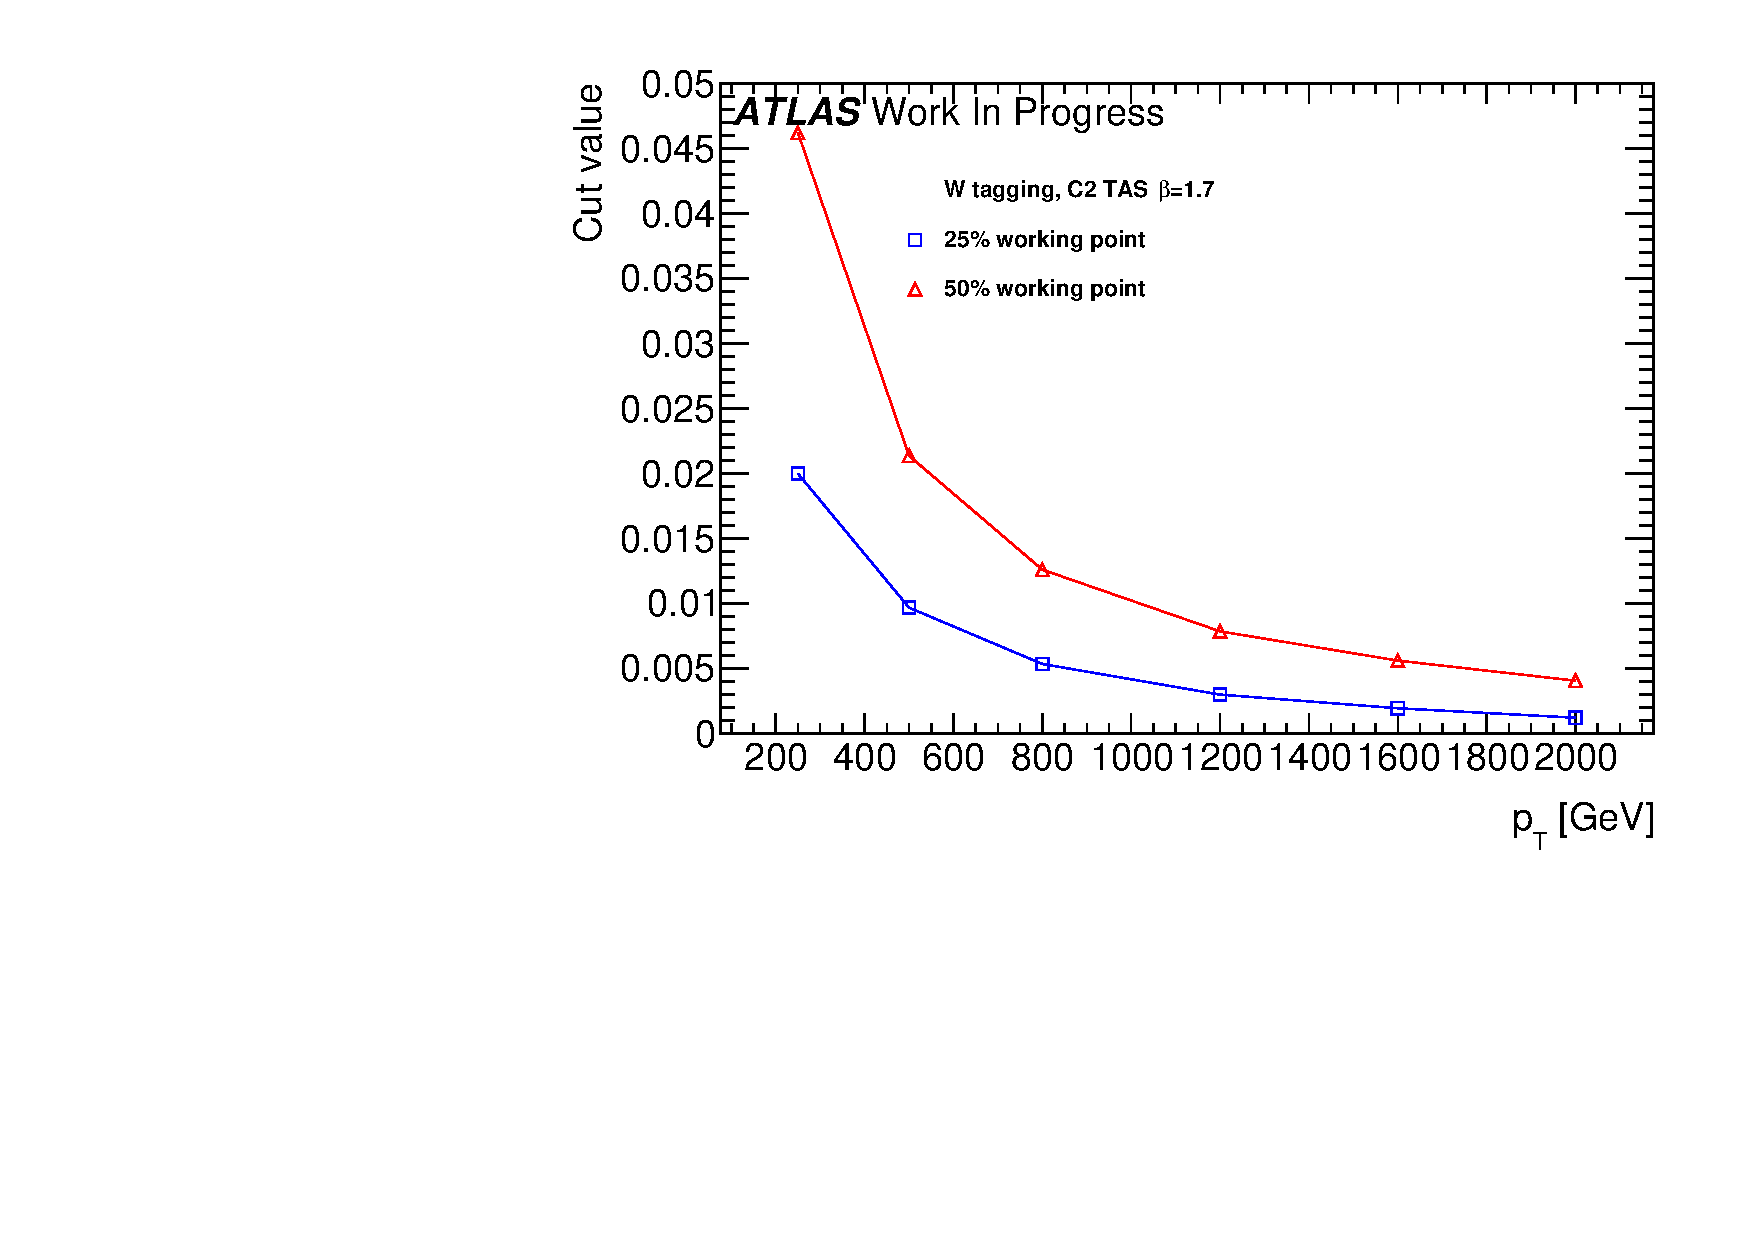
\includegraphics[width=0.5\textwidth]{sascha_input/plots/W/cut_value/c2_tas17.pdf} \hspace{1mm}
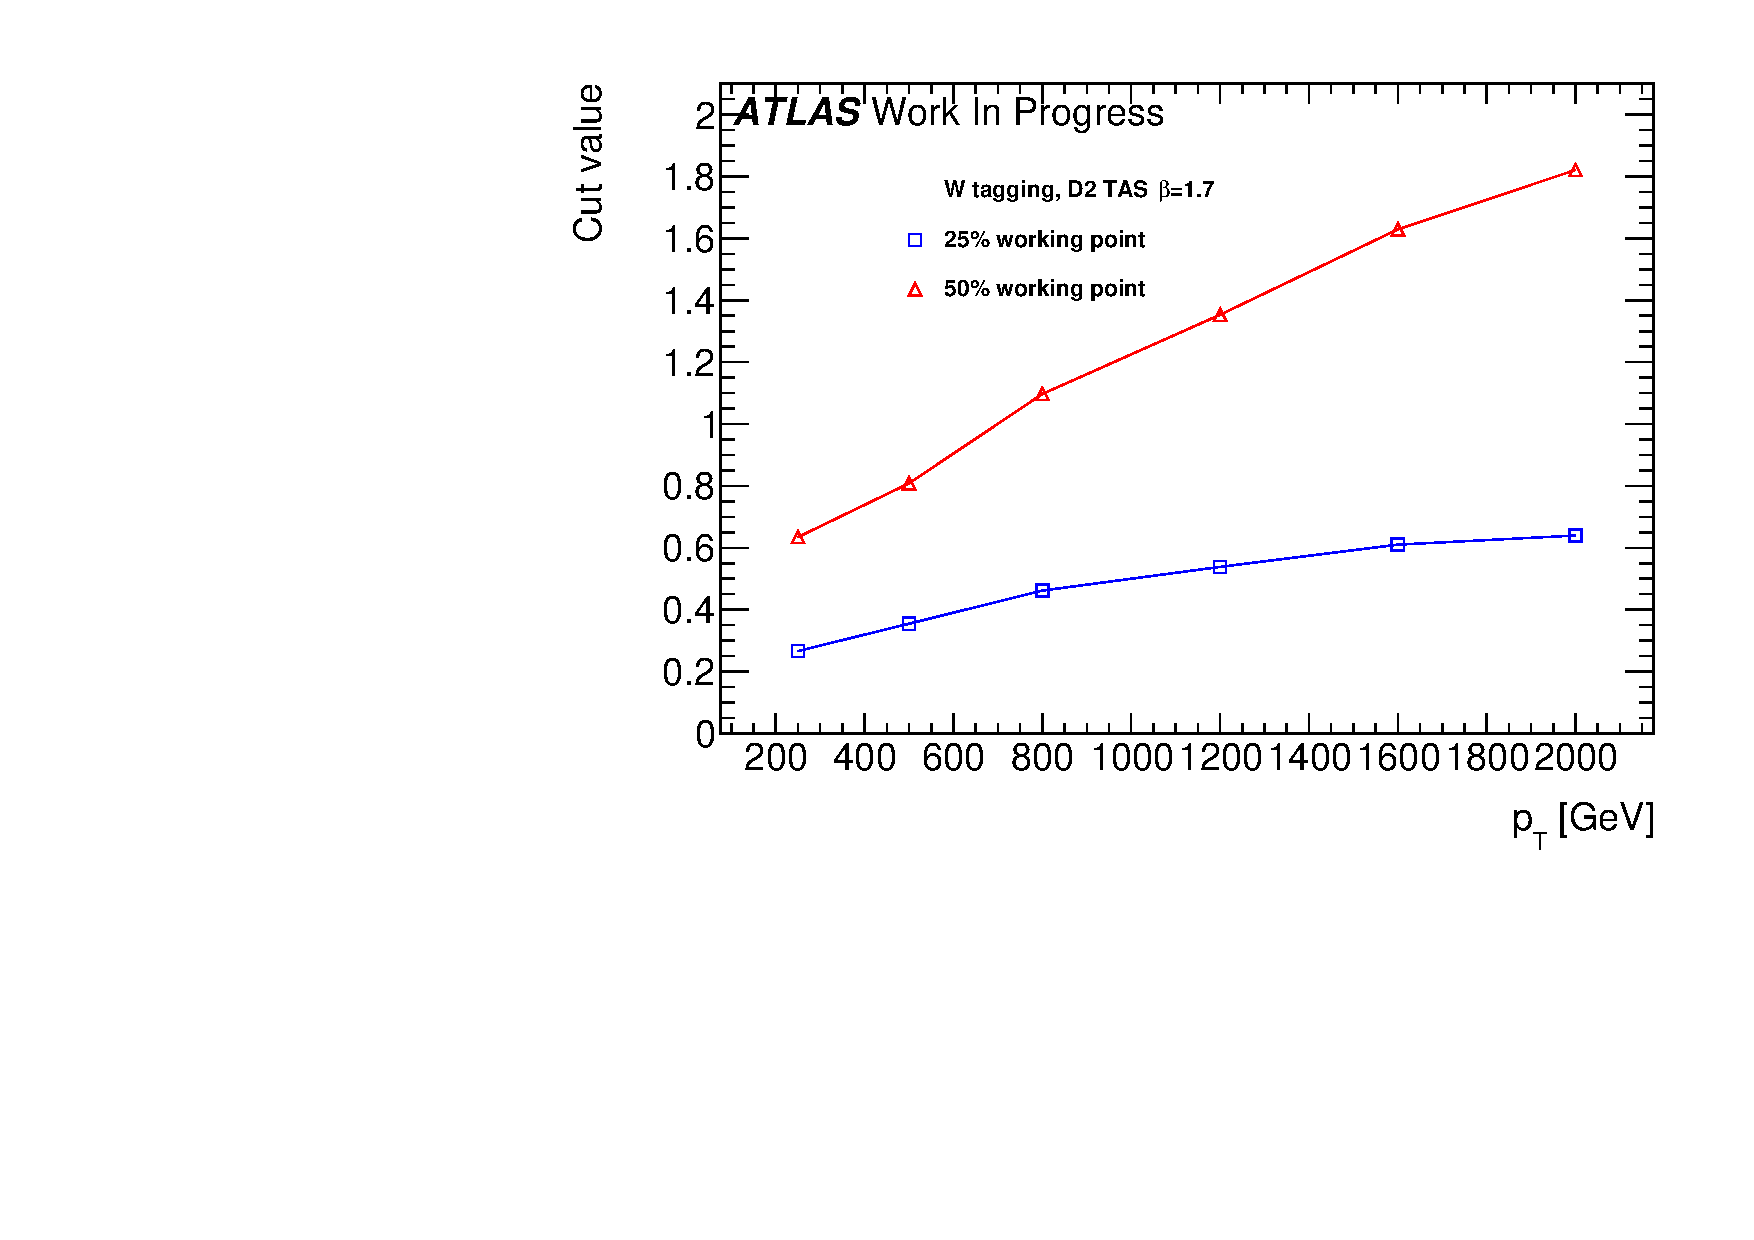
\includegraphics[width=0.5\textwidth]{sascha_input/plots/W/cut_value/d2_tas17.pdf}	
\caption{\footnotesize{Cut values for $\text{C2}_{\text{TAS}}^{(\beta=1.7)}$ (left) and $\text{D2}_{\text{TAS}}^{(\beta=1.7)}$ (right) to achieve $50\,\%$ and $25\,\%$ $W$ boson efficiency.}}\label{fig:w_cut}
\end{figure}
%The steeper $50\,\%$ working point curves can be explained with the signal distributions, see Figure \ref{fig:w_distris}. The signal distributions rise steeply for low values, which doesn't chance considerably with rising $p_{\mathrm{T}}$. The right-handed tail of the distributions in contrast becomes increasingly narrow for $\text{C2}_{\text{TAS}}^{(\beta=1.7)}$ and broader for $\text{D2}_{\text{TAS}}^{(\beta=1.7)}$. Therefore, the curves for the $50\,\%$ cut feature a larger slope as the $25\,\%$ cut, which already given by the sharp rise. 

Table \ref{table:w_improvement} lists the background rejections for $\text{D2}_{\text{TAS}}^{(\beta=1.7)}$, $\text{C2}_{\text{TAS}}^{(\beta=1.7)}$ and the currently used $\text{D2}^{\beta=1}_{calo}$ along with the corresponding improvements. For lower energies, $\text{D2}_{\text{TAS}}^{(\beta=1.7)}$ is the best choice. For very high boosts of the $W$ boson, $\text{C2}_{\text{TAS}}^{(\beta=1.7)}$ performs superior, especially for $25\,\%$ $\epsilon_{signal}$, where the background rejection with $\text{C2}_{\text{TAS}}^{(\beta=1.7)}$ is around 3.5 times as large as the QCD rejection with $\text{D2}^{(\beta=1)}_{\text{calo}}$.
%\begin{figure}[]
%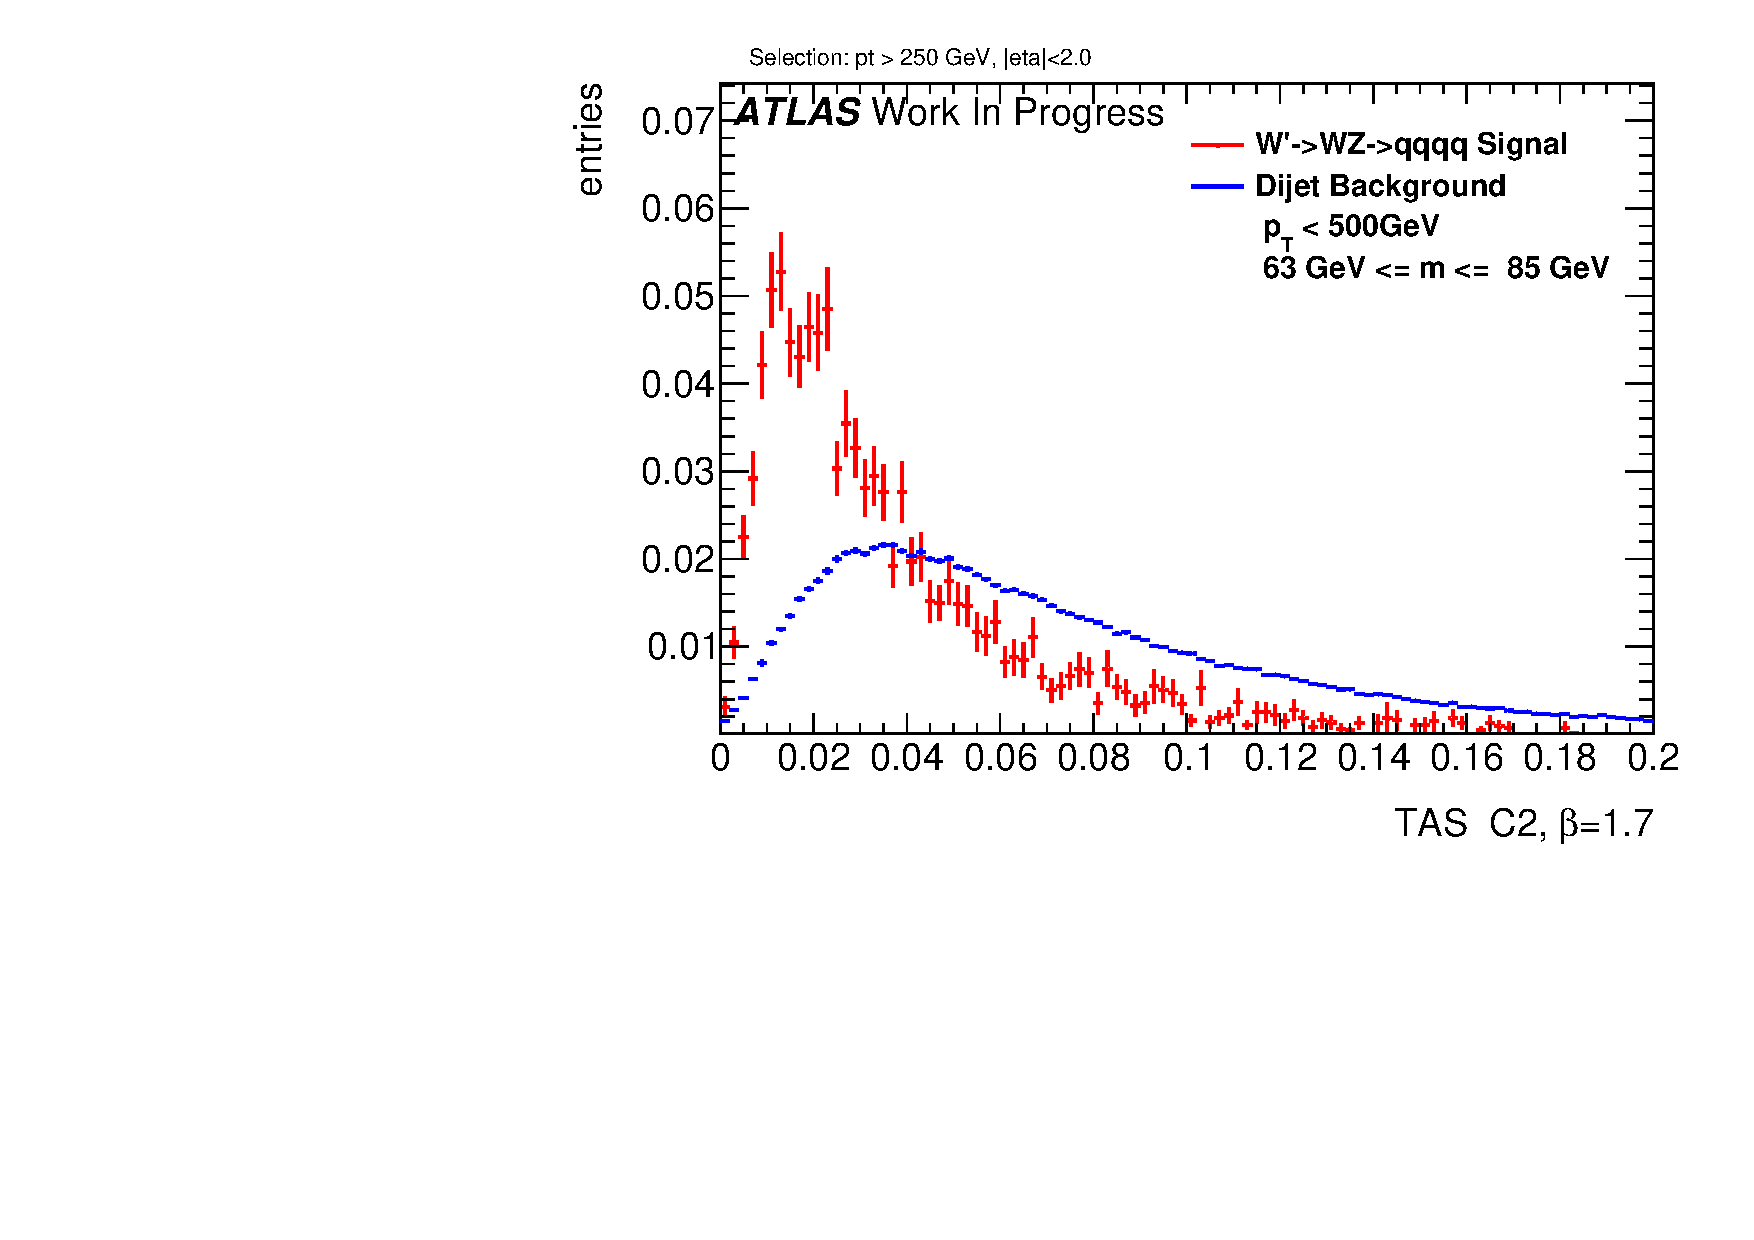
\includegraphics[width=0.25\textwidth]{sascha_input/plots/W/cut_value/h_assisted_tj_C2_17_bin1.pdf} 
%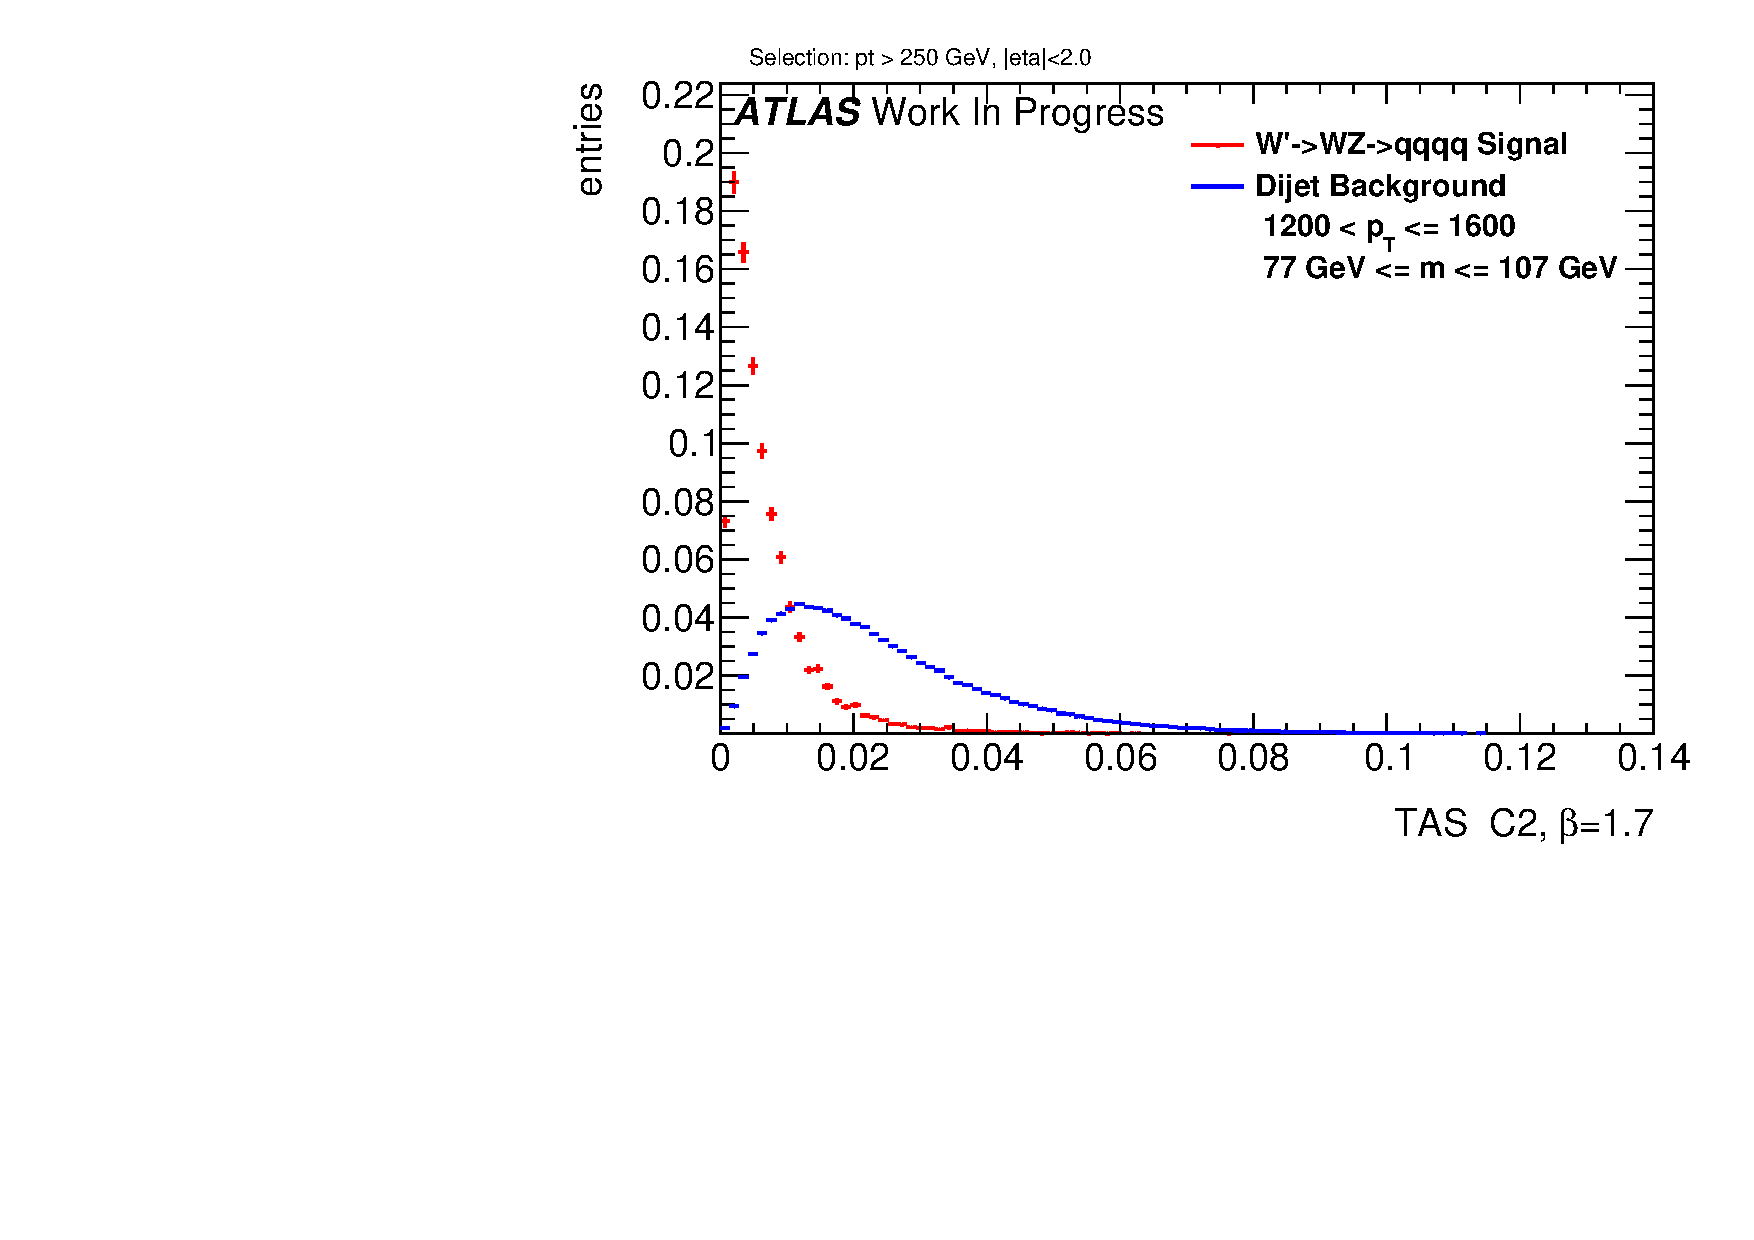
\includegraphics[width=0.25\textwidth]{sascha_input/plots/W/cut_value/h_assisted_tj_C2_17_bin4.pdf} 
%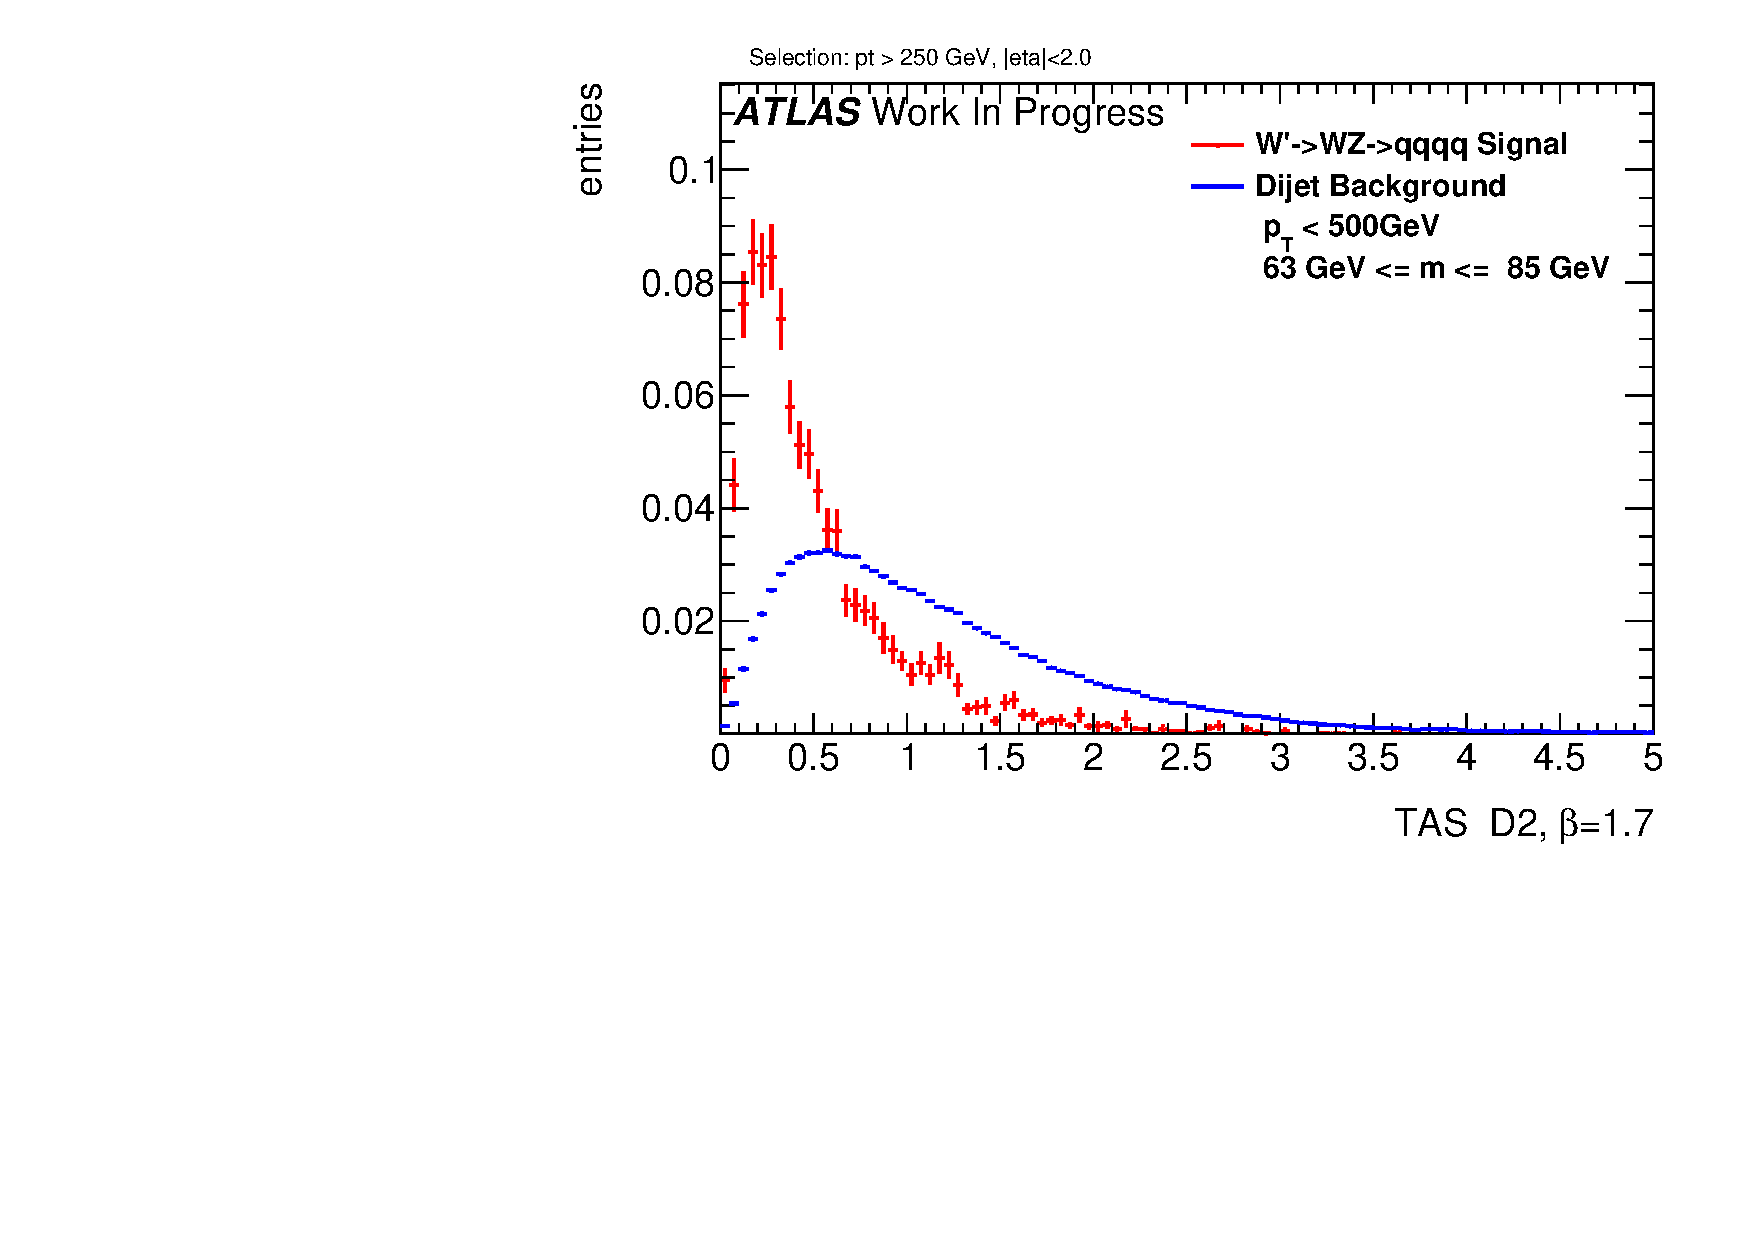
\includegraphics[width=0.25\textwidth]{sascha_input/plots/W/cut_value/h_assisted_tj_D2_17_bin1.pdf} 
%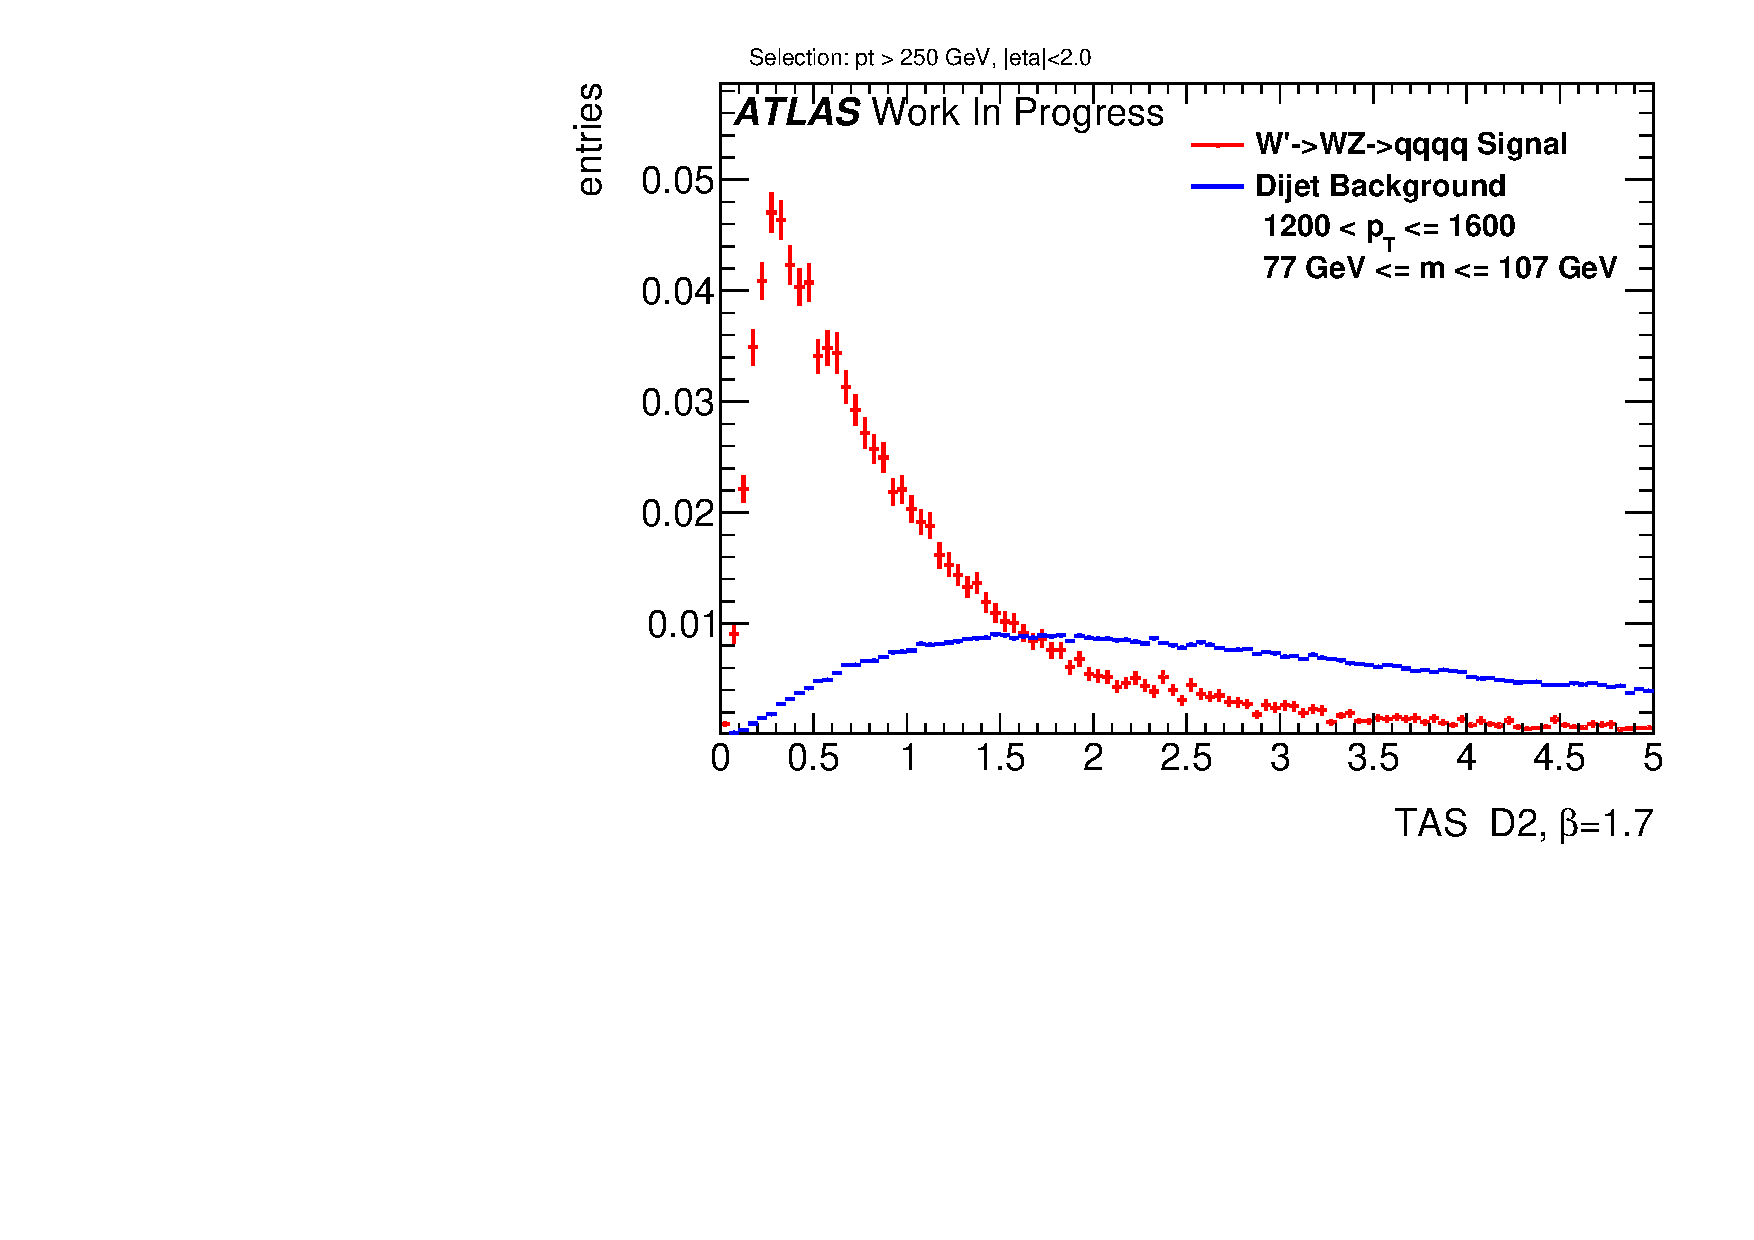
\includegraphics[width=0.25\textwidth]{sascha_input/plots/W/cut_value/h_assisted_tj_D2_17_bin4.pdf} 
%\caption{\footnotesize{$W$ boson signal and QCD background distributions for C2 TAS at $\beta=1.7$ (above) and D2 TAS at $\beta=1.7$ (below) for the %first (left) and fourth (right) $p_{\mathrm{T}}$ bin.}}\label{fig:w_distris}
%\end{figure}
These enormous improvements at lower $\epsilon_{signal}$ are due to the signal distributions for TAS and tracks rising much steeper than for clusters. The tail to higher, background like values in contrast, is more comparable, leading to an alignment of the background rejection for very large $\epsilon_{signal}$. The improvements due to TAS lie around $50\,\%$ for D2 and up to a $100\,\%$ for C2 in the upper $p_{\mathrm{T}}$ regions and $50\,\%$ $W$ boson efficiency. For the lower working point, they can reach $200\,\%$ for D2 and around $250\,\%$ for C2, again for very large boosts of the $W$ boson.
\begin{table}[]
\centering
\begin{tabular}{llll}
 \multicolumn{1}{l||}{\textbf{50\% $\epsilon_{signal}$}} &                                                & \textbf{W tagging}                                         &                                          \\ \hline
\multicolumn{1}{l||}{$p_{\mathrm{T}} \, \text{[GeV]}$}           & \multicolumn{1}{l|}{$\text{D2}_{\text{calo}}^{(\beta=1)}$} & \multicolumn{1}{l|}{$\text{D2}_{\text{TAS}}^{(\beta=1.7)}$} & \multicolumn{1}{l|}{$\text{C2}_{\text{TAS}}^{(\beta=1.7)}$} \\ \hline \hline
\multicolumn{1}{l||}{250 - 500}                       & \multicolumn{1}{l|}{35.0 $\pm$ 2.0}                      & \multicolumn{1}{l|}{35.4 $\pm$ 2.3 (+1 $\pm$ 9\%)}         & \multicolumn{1}{l|}{28.9 $\pm$ 1.5 (-17 $\pm$ 6\%)}        \\
\multicolumn{1}{l||}{500 - 800}                       & \multicolumn{1}{l|}{55.3 $\pm$ 2.6}                      & \multicolumn{1}{l|}{67.6 $\pm$ 3.2 (+22 $\pm$ 8\%)}        & \multicolumn{1}{l|}{58.6 $\pm$ 2.6 (+6 $\pm$ 7\%)}         \\
\multicolumn{1}{l||}{800 - 1200}                      & \multicolumn{1}{l|}{41.1 $\pm$ 2.0}                      & \multicolumn{1}{l|}{54.9 $\pm$ 2.4 (+34 $\pm$ 9\%)}        & \multicolumn{1}{l|}{54.6 $\pm$ 2.8 (+33 $\pm$ 9\%)}        \\
\multicolumn{1}{l||}{1200 - 1600}                     & \multicolumn{1}{l|}{38.1 $\pm$ 1.9}                      & \multicolumn{1}{l|}{50.8 $\pm$ 1.8 (+33 $\pm$ 8\%)}        & \multicolumn{1}{l|}{53.8 $\pm$ 2.7 (+41 $\pm$ 10\%)}        \\
\multicolumn{1}{l||}{1600 - 2000}                     & \multicolumn{1}{l|}{25.4 $\pm$ 1.3}                      & \multicolumn{1}{l|}{37.8 $\pm$ 2.0 (+49 $\pm$ 11\%)}       & \multicolumn{1}{l|}{50.9 $\pm$ 4.3 (+100 $\pm$ 20\%)}       \\
\multicolumn{1}{l||}{$>2000$}                         & \multicolumn{1}{l|}{21.9 $\pm$ 1.7}                      & \multicolumn{1}{l|}{36.3 $\pm$ 2.0 (+66 $\pm$ 16\%)}       & \multicolumn{1}{l|}{46.1 $\pm$ 4.7 (+111 $\pm$ 27\%)}       \\ \hline
                                                     &                                                &                                          &                                          \\
 \multicolumn{1}{l||}{  \textbf{25\% $\epsilon_{signal}$}} &                                                &  \textbf{W tagging}                                         &                                          \\ \hline
\multicolumn{1}{l||}{$p_{\mathrm{T}} \, \text{[GeV]}$}           & \multicolumn{1}{l|}{$\text{D2}_{\text{calo}}^{(\beta=1)}$} & \multicolumn{1}{l|}{$\text{D2}_{\text{TAS}}^{(\beta=1.7)}$} & \multicolumn{1}{l|}{$\text{C2}_{\text{TAS}}^{(\beta=1.7)}$} \\ \hline \hline
\multicolumn{1}{l||}{250 - 500}                       & \multicolumn{1}{l|}{139.6 $\pm$ 9.8}                     	& \multicolumn{1}{l|}{146.0 $\pm$ 12.4 (+5 $\pm$ 12\%)}         & \multicolumn{1}{l|}{108.2 $\pm$ 7.5 (-22 $\pm$ 8\%)}       \\
\multicolumn{1}{l||}{500 - 800}                       & \multicolumn{1}{l|}{243.7 $\pm$ 13.2}                     	& \multicolumn{1}{l|}{360.1 $\pm$ 21.1 (+48 $\pm$ 12\%)}        & \multicolumn{1}{l|}{298.4 $\pm$ 15.9 (+22 $\pm$ 9\%)}        \\
\multicolumn{1}{l||}{800 -1200}                       & \multicolumn{1}{l|}{181.0 $\pm$ 8.8}                     	& \multicolumn{1}{l|}{308.5 $\pm$ 19.3 (+70 $\pm$ 14\%)}        & \multicolumn{1}{l|}{313.2 $\pm$ 24.4 (+78 $\pm$ 16\%)}       \\
\multicolumn{1}{l||}{1200 - 1600}                     & \multicolumn{1}{l|}{156.9 $\pm$ 8.3}                     	& \multicolumn{1}{l|}{295.4 $\pm$ 17.8 (+88 $\pm$ 15\%)}        & \multicolumn{1}{l|}{354.6 $\pm$ 25.6 (+126 $\pm$ 20\%)}      \\
\multicolumn{1}{l||}{1600 - 2000}                     & \multicolumn{1}{l|}{84.6 $\pm$ 5.7}                      	& \multicolumn{1}{l|}{219.6 $\pm$ 10.9 (+160 $\pm$ 22\%)}       & \multicolumn{1}{l|}{320.5 $\pm$ 31.4 (+279 $\pm$ 45\%)}       \\
\multicolumn{1}{l||}{$>2000$}                         & \multicolumn{1}{l|}{78.9 $\pm$ 7.6}                      	& \multicolumn{1}{l|}{233.5 $\pm$ 14.7 (+196 $\pm$ 34\%)}       & \multicolumn{1}{l|}{288.4 $\pm$ 33.3 (+266 $\pm$ 55\%)}      \\ \hline
\end{tabular}

\caption{Listing of the background rejections after the jet mass cut and tagging at 50\% and 25\% $W$ boson efficiency for the identified best variables $\text{D2}_{\text{TAS}}^{(\beta=1.7)}$ \& $\text{C2}_{\text{TAS}}^{(\beta=1.7)}$ together with the improvements over the standard choice $\text{D2}_{\text{calo}}^{(\beta=1)}$}\label{table:w_improvement}
\end{table}



\subsubsection{Optimisation for Higgs boson jets}
The results of the optimisation for Higgs boson jets are shown in Table \ref{table:higgs_scan}. The study of $\beta=1$ in the Higgs boson case, see section \ref{subsubsec:higgs_beta1}, showed no improvements in the rejection of QCD events due to tracks and TAS as input. As for the $W$ boson, the performance of tracks and TAS diminishes considerably with an angular weighting of $\beta=0.5$.

No improvement of $\tau_{21}$ is observed with tracks or TAS, clusters perform equally well for lower $p_{\mathrm{T}}$ and slightly better at high energies. Again, the QCD rejection achieved with $\tau_{21}$ is exceeded by C2 and D2. The discrimination with clusters profits from a slightly higher angular weighting, although the gain is not as significant as for tracks and TAS. This consistently shows the lower sensitivity to a variation of the angular weight. The small gain is connected to the higher separation of the Higgs decay products compared to the $W$ boson case.

For boosted Higgs tagging, D2 outperforms C2 over the whole studied energy range. Values of $\beta=1.7 \& 2$ yield the highest background rejection for track and TAS based D2. $\text{D2}_{\text{TAS}}^{(\beta=1.7,2}$ and $\text{D2}_{\text{track}}^{(\beta=1.7,2}$ perform superior to $\text{D2}_{\text{calo}}$ at high boosts, due to the low angular separation of constituents, and equally well at lower enegies.

The differences between $\beta=1.7$ and $\beta=2$ are inconclusive with minor advantages at high and slight inferiorities at low $p_{\mathrm{T}}$ for $\beta=2$. Tracks perform slightly worse than TAS for lower energies but similarly better in the two highest studied $p_{\mathrm{T}}$ regions. Chosen for further examination are $\text{D2}_{\text{TAS}^{(\beta=1.7)}}$ and $\text{D2}_{\text{track}^{(\beta=1.7)}}$.

\begin{sidewaystable}[]
\centering
\hspace{-1cm}
\resizebox{22cm}{!}{%
\begin{tabular}{llllllllllllllll}
 \multicolumn{1}{l||}{\textbf{Calorimeter}}    &                                  &                           & C2                        &                           & \multicolumn{1}{l|}{}     &                                  &                           & D2                        &                           & \multicolumn{1}{l|}{}     &                                  &                           & $\tau_{21}$               &                           & \multicolumn{1}{l|}{}     \\ \hline
\multicolumn{1}{l||}{$p_{\mathrm{T}} \, [GeV]$} & \multicolumn{1}{l|}{$\beta=0.5$} & \multicolumn{1}{l|}{1}    & \multicolumn{1}{l|}{1.7}  & \multicolumn{1}{l|}{2}    & \multicolumn{1}{l||}{3}    & \multicolumn{1}{l|}{$\beta=0.5$} & \multicolumn{1}{l|}{1}    & \multicolumn{1}{l|}{1.7}  & \multicolumn{1}{l|}{2}    & \multicolumn{1}{l||}{3}    & \multicolumn{1}{l|}{$\beta=0.5$} & \multicolumn{1}{l|}{1}    & \multicolumn{1}{l|}{1.7}  & \multicolumn{1}{l|}{2}    & \multicolumn{1}{l|}{3}    \\ \hline \hline
\multicolumn{1}{l||}{250 - 500}      & \multicolumn{1}{l|}{4.6(0.1)}         & \multicolumn{1}{l|}{5.0(0.1)} & \multicolumn{1}{l|}{5.2(0.1)}  	    & \multicolumn{1}{l|}{5.3(0.1)}  & \multicolumn{1}{l||}{5.5(0.1)}  		& \multicolumn{1}{l|}{5.7(0.1)}         & \multicolumn{1}{l|}{7.3(0.2)}  & \multicolumn{1}{l|}{8.4(0.2)}  							& \multicolumn{1}{l|}{8.4(0.2)}  	    & \multicolumn{1}{l||}{8.4(0.2)}  & \multicolumn{1}{l|}{7.6(0.2)}         & \multicolumn{1}{l|}{8.0(0.2)}  & \multicolumn{1}{l|}{7.9(0.2)}  & \multicolumn{1}{l|}{7.8(0.2)}  & \multicolumn{1}{l|}{7.5(0.2)}  \\
\multicolumn{1}{l||}{500 - 800}      & \multicolumn{1}{l|}{15.7(0.3)}        & \multicolumn{1}{l|}{16.7(0.4)} & \multicolumn{1}{l|}{17.0(0.4)} 		& \multicolumn{1}{l|}{16.9(0.4)} & \multicolumn{1}{l||}{16.2(0.4)} 		& \multicolumn{1}{l|}{13.6(0.3)}        & \multicolumn{1}{l|}{16.9(0.4)} & \multicolumn{1}{l|}{17.7(0.4)} 		& \multicolumn{1}{l|}{17.2(0.4)} 						& \multicolumn{1}{l||}{15.2(0.3)} & \multicolumn{1}{l|}{16.7(0.4)}        & \multicolumn{1}{l|}{15.4(0.3)} & \multicolumn{1}{l|}{15.2(0.3)} & \multicolumn{1}{l|}{14.8(0.3)} & \multicolumn{1}{l|}{14.0(0.3)} \\
\multicolumn{1}{l||}{800 - 1200}     & \multicolumn{1}{l|}{22.1(0.5)}        & \multicolumn{1}{l|}{23.8(0.5)} & \multicolumn{1}{l|}{25.0(0.6)} 		& \multicolumn{1}{l|}{25.0(0.6)} & \multicolumn{1}{l||}{23.4(0.5)} 		& \multicolumn{1}{l|}{18.4(0.4)}        & \multicolumn{1}{l|}{23.7(0.6)} & \multicolumn{1}{l|}{26.3(0.6)} 							& \multicolumn{1}{l|}{25.6(0.6)} 		& \multicolumn{1}{l||}{22.3(0.5)} & \multicolumn{1}{l|}{22.8(0.5)}        & \multicolumn{1}{l|}{21.9(0.5)} & \multicolumn{1}{l|}{22.6(0.5)} & \multicolumn{1}{l|}{22.1(0.5)} & \multicolumn{1}{l|}{20.9(0.5)} \\
\multicolumn{1}{l||}{1200 - 1600}    & \multicolumn{1}{l|}{24.0(0.6)}        & \multicolumn{1}{l|}{26.0(0.8)} & \multicolumn{1}{l|}{26.4(0.8)} 		& \multicolumn{1}{l|}{25.9(0.7)} & \multicolumn{1}{l||}{23.0(0.6)} 		& \multicolumn{1}{l|}{19.3(0.6)}        & \multicolumn{1}{l|}{24.9(0.7)} & \multicolumn{1}{l|}{27.0(0.8)} 		& \multicolumn{1}{l|}{26.1(0.7)} 						& \multicolumn{1}{l||}{21.9(0.5)} & \multicolumn{1}{l|}{21.3(0.5)}        & \multicolumn{1}{l|}{22.6(0.6)} & \multicolumn{1}{l|}{24.0(0.6)} & \multicolumn{1}{l|}{23.7(0.6)} & \multicolumn{1}{l|}{22.2(0.5)} \\
\multicolumn{1}{l||}{1600 - 2000}    & \multicolumn{1}{l|}{12.1(0.7)}        & \multicolumn{1}{l|}{13.9(0.8)} & \multicolumn{1}{l|}{14.3(0.7)}  	& \multicolumn{1}{l|}{14.0(0.7)} & \multicolumn{1}{l||}{12.3(0.6)} 		& \multicolumn{1}{l|}{11.1(0.7)}        & \multicolumn{1}{l|}{14.1(0.9)} & \multicolumn{1}{l|}{14.9(0.8)} 		& \multicolumn{1}{l|}{14.2(0.6)} 						& \multicolumn{1}{l||}{11.8(0.5)} & \multicolumn{1}{l|}{10.3(0.5)}        & \multicolumn{1}{l|}{11.9(0.5)} & \multicolumn{1}{l|}{13.1(0.6)} & \multicolumn{1}{l|}{13.1(0.7)} & \multicolumn{1}{l|}{12.3(0.7)} \\ \hline
                                    &                                  &                           &                           &                	           &                           &                                  &                           &                           &                           &                           &                                  &                           &                           &                           &                           \\
\multicolumn{1}{l||}{\textbf{TAS}}            &                                  &                           & C2                        &                           & \multicolumn{1}{l|}{}     &                                  &                           & D2                        &                           & \multicolumn{1}{l|}{}     &                                  &                           & $\tau_{21}$               &                           & \multicolumn{1}{l|}{}     \\ \hline
\multicolumn{1}{l||}{$p_{\mathrm{T}} \, [GeV]$} & \multicolumn{1}{l|}{$\beta=0.5$} & \multicolumn{1}{l|}{1}        & \multicolumn{1}{l|}{1.7}    & \multicolumn{1}{l|}{2}    & \multicolumn{1}{l||}{3}    & \multicolumn{1}{l|}{$\beta=0.5$} & \multicolumn{1}{l|}{1}    & \multicolumn{1}{l|}{1.7}  & \multicolumn{1}{l|}{2}    & \multicolumn{1}{l||}{3}    & \multicolumn{1}{l|}{$\beta=0.5$} & \multicolumn{1}{l|}{1}    & \multicolumn{1}{l|}{1.7}  & \multicolumn{1}{l|}{2}    & \multicolumn{1}{l|}{3}    \\ \hline \hline
\multicolumn{1}{l||}{250 - 500}      & \multicolumn{1}{l|}{4.8(0.1)}         & \multicolumn{1}{l|}{5.2(0.1)}  & \multicolumn{1}{l|}{5.5(0.1)}        & \multicolumn{1}{l|}{5.6(0.1)}  				& \multicolumn{1}{l||}{5.8(0.1)}    & \multicolumn{1}{l|}{5.9(0.1)}         	& \multicolumn{1}{l|}{7.6(0.2)}  	& \multicolumn{1}{l|}{8.5(0.2)}  	& \multicolumn{1}{l|}{8.6(0.2)}  		        & \multicolumn{1}{l||}{8.5(0.2)}  							& \multicolumn{1}{l|}{7.6(0.2)}         & \multicolumn{1}{l|}{8.0(0.2)}  &   \multicolumn{1}{l|}{7.7(0.2)}  &   \multicolumn{1}{l|}{7.6(0.2)}  & \multicolumn{1}{l|}{7.4(0.2)}  \\
\multicolumn{1}{l||}{500 - 800}      & \multicolumn{1}{l|}{16.1(0.4)}        & \multicolumn{1}{l|}{17.3(0.4)} & \multicolumn{1}{l|}{17.7(0.4)} 	     & \multicolumn{1}{l|}{17.7(0.4)} 				& \multicolumn{1}{l||}{17.6(0.4)} 	& \multicolumn{1}{l|}{14.0(0.3)}        	& \multicolumn{1}{l|}{18.2(0.4)} 	& \multicolumn{1}{l|}{18.7(0.4)} 		& \multicolumn{1}{l|}{18.3(0.4)} 						& \multicolumn{1}{l||}{16.9(0.4)} 							& \multicolumn{1}{l|}{16.2(0.4)}        & \multicolumn{1}{l|}{16.4(0.4)} & 	 \multicolumn{1}{l|}{15.4(0.4)} & 	\multicolumn{1}{l|}{15.1(0.3)} & \multicolumn{1}{l|}{14.6(0.3)} \\
\multicolumn{1}{l||}{800 - 1200}     & \multicolumn{1}{l|}{20.6(0.5)}        & \multicolumn{1}{l|}{23.5(0.5)} & \multicolumn{1}{l|}{26.2(0.6)} 		 & \multicolumn{1}{l|}{26.9(0.7)} 				& \multicolumn{1}{l||}{27.7(0.6)} 	& \multicolumn{1}{l|}{18.8(0.4)}        	& \multicolumn{1}{l|}{25.6(0.6)} 	& \multicolumn{1}{l|}{28.5(0.7)} 		& \multicolumn{1}{l|}{28.4(0.7)} 						& \multicolumn{1}{l||}{26.8(0.6)} 							& \multicolumn{1}{l|}{21.7(0.5)}        & \multicolumn{1}{l|}{22.4(0.5)} & 	 \multicolumn{1}{l|}{22.1(0.5)} & 	\multicolumn{1}{l|}{22.0(0.5)} & \multicolumn{1}{l|}{21.8(0.5)} \\
\multicolumn{1}{l||}{1200 - 1600}    & \multicolumn{1}{l|}{18.6(0.4)}        & \multicolumn{1}{l|}{22.6(0.6)} & \multicolumn{1}{l|}{27.4(0.7)} 		 & \multicolumn{1}{l|}{28.7(0.8)} 				& \multicolumn{1}{l||}{30.0(0.7)} 	& \multicolumn{1}{l|}{17.9(0.4)}        	& \multicolumn{1}{l|}{24.3(0.7)} 	& \multicolumn{1}{l|}{28.9(0.7)} 						& \multicolumn{1}{l|}{29.3(0.6)} 		& \multicolumn{1}{l||}{28.1(0.7)} 							& \multicolumn{1}{l|}{19.3(0.5)}        & \multicolumn{1}{l|}{20.0(0.5)} & 	 \multicolumn{1}{l|}{20.7(0.5)} & 	\multicolumn{1}{l|}{21.0(0.6)} & \multicolumn{1}{l|}{21.9(0.5)} \\
\multicolumn{1}{l||}{1600 - 2000}    & \multicolumn{1}{l|}{8.0(0.3)}         & \multicolumn{1}{l|}{11.3(0.5)} & \multicolumn{1}{l|}{15.4(0.9)} 		 & \multicolumn{1}{l|}{16.5(1.0)} 				& \multicolumn{1}{l||}{17.8(0.7)} 	& \multicolumn{1}{l|}{10.0(0.5)}        	& \multicolumn{1}{l|}{14.0(0.8)} 	& \multicolumn{1}{l|}{17.7(0.8)} 						& \multicolumn{1}{l|}{18.1(.9)} 		& \multicolumn{1}{l||}{17.9(0.6)} 							& \multicolumn{1}{l|}{9.8(0.4)}         & \multicolumn{1}{l|}{10.6(0.5)} & 	 \multicolumn{1}{l|}{11.4(0.6)} & 	\multicolumn{1}{l|}{11.8(0.6)} & \multicolumn{1}{l|}{12.6(0.6)} \\ \hline
                                    &                                  &                           &                           &                           &                           &                                  &                           &                           &                           &                           &                                  &                           &                           &                           &                           \\
 \multicolumn{1}{l||}{\textbf{Tracks}}         &                                  &                           & C2                        &                           & \multicolumn{1}{l|}{}     &                                  &                           & D2                        &                           & \multicolumn{1}{l|}{}     &                                  &                           & $\tau_{21}$               &                           & \multicolumn{1}{l|}{}     \\ \hline
\multicolumn{1}{l||}{$p_{\mathrm{T}} \, [GeV]$} & \multicolumn{1}{l|}{$\beta=0.5$} & \multicolumn{1}{l|}{1}    & \multicolumn{1}{l|}{1.7}  & \multicolumn{1}{l|}{2}    & \multicolumn{1}{l||}{3}    & \multicolumn{1}{l|}{$\beta=0.5$} & \multicolumn{1}{l|}{1}    & \multicolumn{1}{l|}{1.7}  & \multicolumn{1}{l|}{2}    & \multicolumn{1}{l||}{3}    & \multicolumn{1}{l|}{$\beta=0.5$} & \multicolumn{1}{l|}{1}    & \multicolumn{1}{l|}{1.7}  & \multicolumn{1}{l|}{2}    & \multicolumn{1}{l|}{3}    \\ \hline \hline
\multicolumn{1}{l||}{250 - 500}      & \multicolumn{1}{l|}{4.91(0.1)}       & \multicolumn{1}{l|}{5.2(0.1)}  		& \multicolumn{1}{l|}{5.5(0.1)}  		& \multicolumn{1}{l|}{5.6(0.1)}  								& \multicolumn{1}{l||}{5.9(0.1)}  					    & \multicolumn{1}{l|}{5.8(0.1)}         	& \multicolumn{1}{l|}{7.4(0.2)}  	& \multicolumn{1}{l|}{8.3(0.2)} 				 		& \multicolumn{1}{l|}{8.3(0.2)}  					& \multicolumn{1}{l||}{8.5(0.2)}  	& \multicolumn{1}{l|}{7.4(0.2)}         & \multicolumn{1}{l|}{7.9(0.2)}  	& \multicolumn{1}{l|}{7.8(0.2)}  	& \multicolumn{1}{l|}{7.7(0.2)}  	& \multicolumn{1}{l|}{7.6(0.2)}  \\
\multicolumn{1}{l||}{500 - 800}      & \multicolumn{1}{l|}{15.6(0.3)}        & \multicolumn{1}{l|}{17.2(0.4)} 		& \multicolumn{1}{l|}{17.8(0.4)} 		& \multicolumn{1}{l|}{17.9(0.4)} 				& \multicolumn{1}{l||}{17.7(0.4)} 						& \multicolumn{1}{l|}{13.5(0.3)}        	& \multicolumn{1}{l|}{17.1(0.4)} 	& \multicolumn{1}{l|}{17.9(0.4)}		& \multicolumn{1}{l|}{17.7(0.4)} 					& \multicolumn{1}{l||}{16.8(0.4)} 						& \multicolumn{1}{l|}{15.7(0.3)}        & \multicolumn{1}{l|}{16.1(0.4)} 	& \multicolumn{1}{l|}{15.5(0.3)} 	& \multicolumn{1}{l|}{15.3(0.3)} 	& \multicolumn{1}{l|}{14.8(0.1)} \\
\multicolumn{1}{l||}{800 - 1200}     & \multicolumn{1}{l|}{20.1(0.5)}        & \multicolumn{1}{l|}{24.0(0.5)} 		& \multicolumn{1}{l|}{26.9(0.6)} 		& \multicolumn{1}{l|}{27.7(0.7)} 								& \multicolumn{1}{l||}{28.4(0.6)} 	& \multicolumn{1}{l|}{18.8(0.4)}        	& \multicolumn{1}{l|}{25.3(0.6)} 	& \multicolumn{1}{l|}{28.0(0.7)} 						& \multicolumn{1}{l|}{28.0(0.7)} 					& \multicolumn{1}{l||}{26.9(0.6)} 						& \multicolumn{1}{l|}{22.0(0.5)}        & \multicolumn{1}{l|}{22.7(0.5)} 	& \multicolumn{1}{l|}{22.5(0.5)} 	& \multicolumn{1}{l|}{22.4(0.5)} 	& \multicolumn{1}{l|}{22.4(0.3)} \\
\multicolumn{1}{l||}{1200 - 1600}    & \multicolumn{1}{l|}{18.5(0.5)}        & \multicolumn{1}{l|}{23.8(0.6)} 		& \multicolumn{1}{l|}{28.8(0.8)} 		& \multicolumn{1}{l|}{30.0(0.8)} 								& \multicolumn{1}{l||}{31.1(0.7)} 						& \multicolumn{1}{l|}{19.4(0.5)}        	& \multicolumn{1}{l|}{26.3(0.7)} 	& \multicolumn{1}{l|}{30.0(0.8)} 						& \multicolumn{1}{l|}{30.3(0.8)} 	& \multicolumn{1}{l||}{29.2(0.7)} 						& \multicolumn{1}{l|}{20.8(0.5)}        & \multicolumn{1}{l|}{21.4(0.5)} 	& \multicolumn{1}{l|}{21.9(0.6)} 	& \multicolumn{1}{l|}{22.3(0.6)} 	& \multicolumn{1}{l|}{23.0(0.5)} \\
\multicolumn{1}{l||}{1600 - 2000}    & \multicolumn{1}{l|}{8.0(0.3)}         & \multicolumn{1}{l|}{11.7(0.5)} 		& \multicolumn{1}{l|}{16.1(0.9)} 		& \multicolumn{1}{l|}{17.1(0.9)} 								& \multicolumn{1}{l||}{18.3(0.9)} 						& \multicolumn{1}{l|}{11.0(0.7)}        	& \multicolumn{1}{l|}{15.5(0.7)} 	& \multicolumn{1}{l|}{18.5(0.8)} 						& \multicolumn{1}{l|}{18.7(0.8)} 	& \multicolumn{1}{l||}{18.4(0.6)} 						& \multicolumn{1}{l|}{10.4(0.5)}        & \multicolumn{1}{l|}{11.1(0.5)} 	& \multicolumn{1}{l|}{12.0(0.6)} 	& \multicolumn{1}{l|}{12.4(0.7)} 	& \multicolumn{1}{l|}{13.2(0.6)} \\ \hline
\end{tabular}}
\caption{Listing of the QCD background rejection for Higgs signal achieved with C2, D2 and $\tau_{21}$ together with different angular weightings $\beta$ and for calorimeter cluster, tracks and TAS.}\label{table:higgs_scan}
\end{sidewaystable}

Shown in Figure \ref{fig:higgs_cut} are the cut values for $50\,\%$ and $25\,\%$ signal efficiency for $\text{D2}_{\text{TAS}}^{(\beta=1.7)}$ and $\text{D2}_{\text{track}}^{(\beta=1.7)}$. The cut value shows a slight upward trend for rising $p_{\mathrm{T}}$. Moreover, cut values for the first bin are higher as for the second, in contrast to the overall upward trend of D2. This is the result of the low boost in the lowest $p_{\mathrm{T}}$ region resulting in a left shoulder of the mass distributions representing large-R jets containing only part of the Higgs boson decay. These jets feature one-prong structure and result in background-like D2 values. The TAS D2 cut is marginally higher than the corresponding track D2 cut since the assisted tracks have a higher $p_{\mathrm{T}}$ and the D2 cut features a rising tendency with $p_{\mathrm{T}}$. 
\begin{figure}
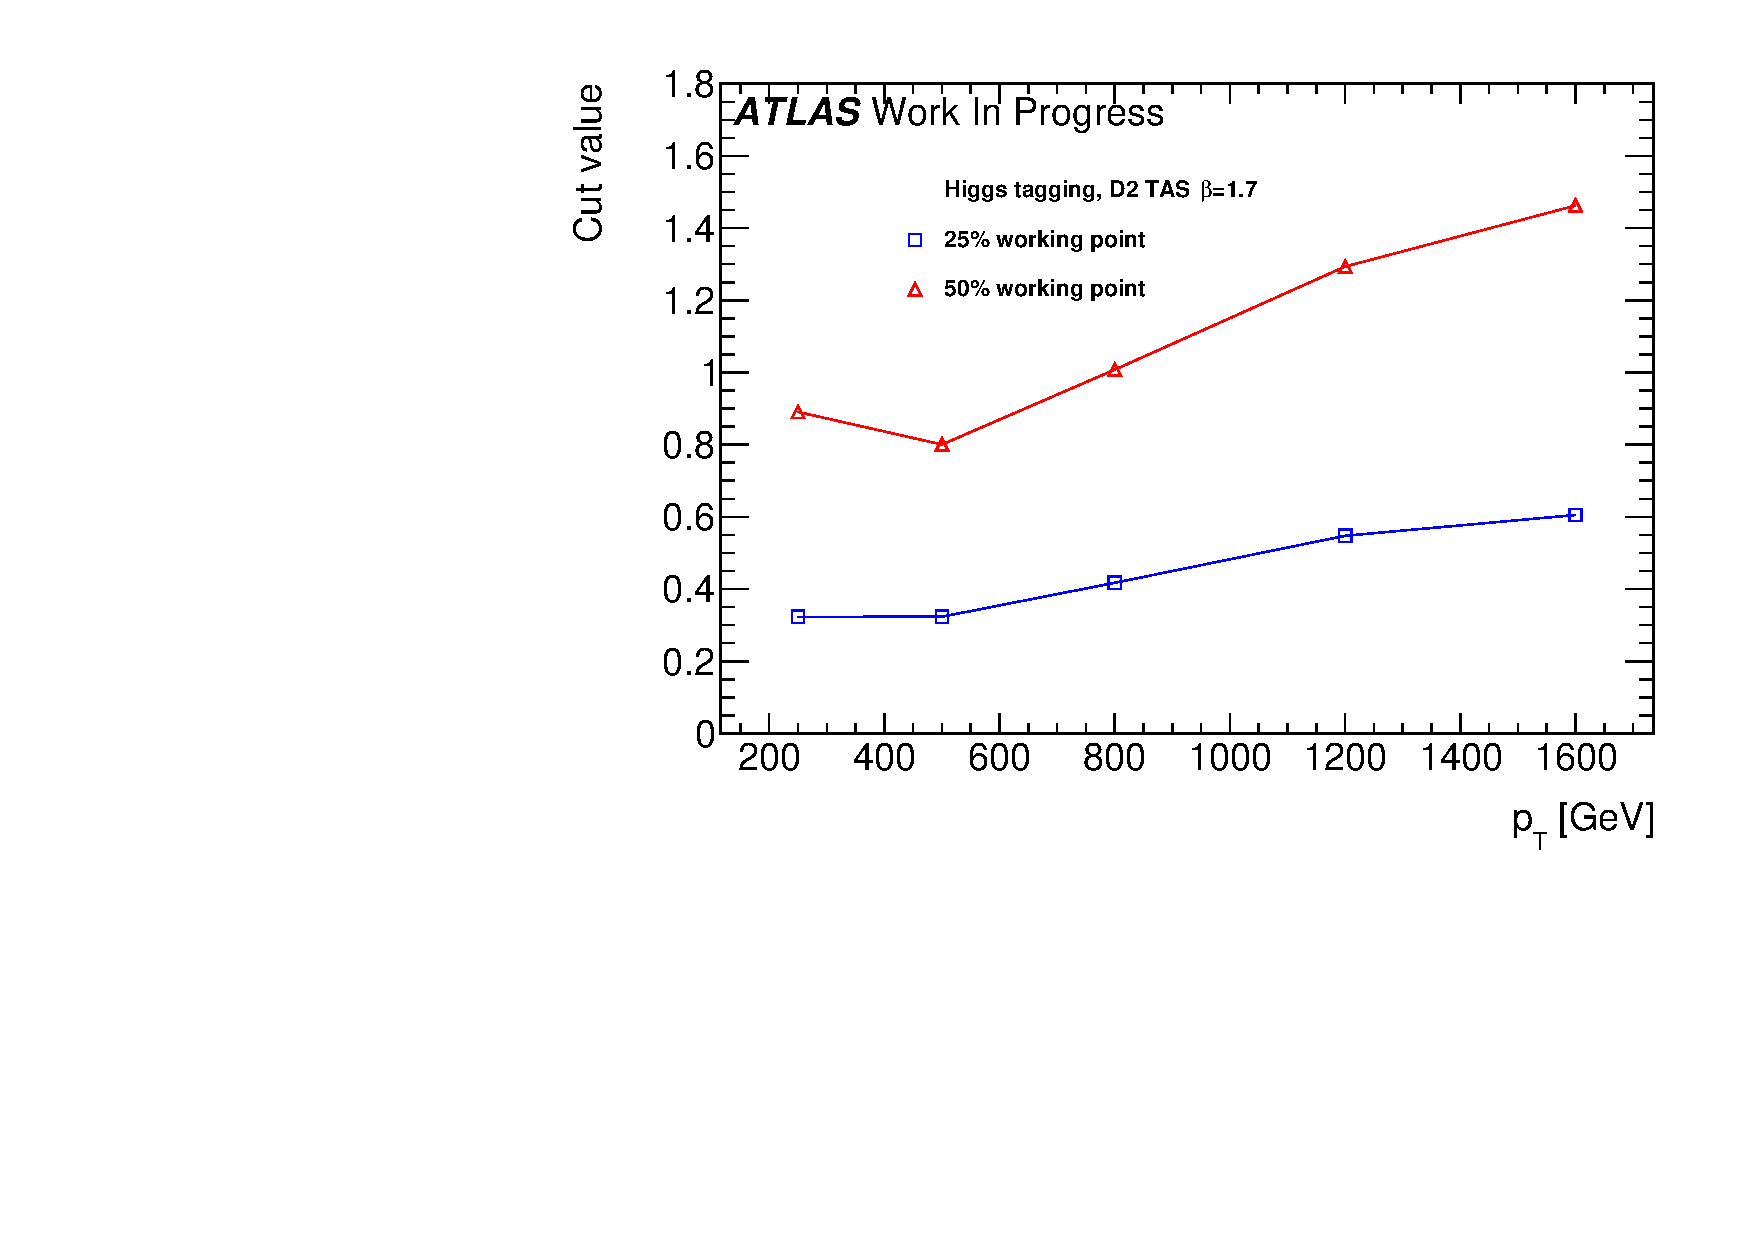
\includegraphics[width=0.5\textwidth]{sascha_input/plots/Higgs/cut_value/d2_tas17.pdf} \hspace{1mm}
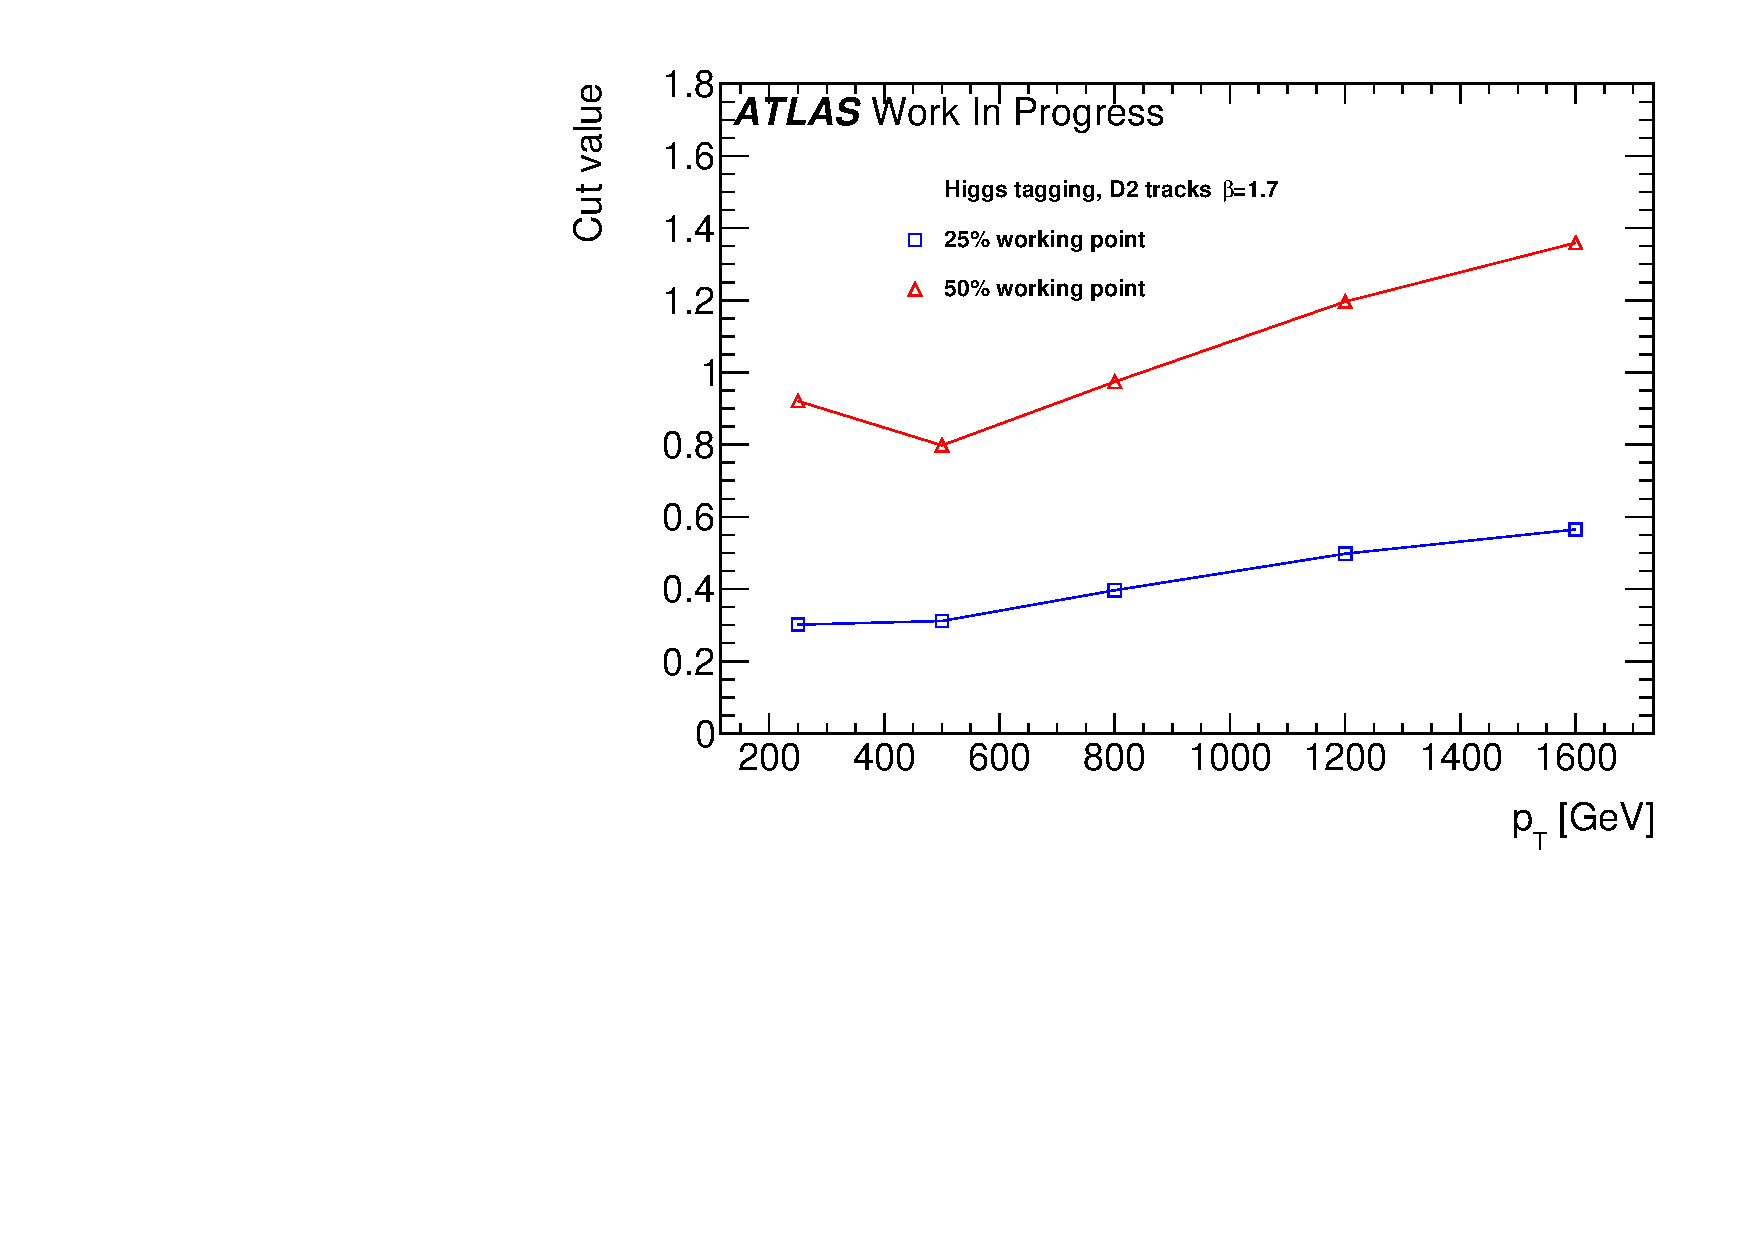
\includegraphics[width=0.5\textwidth]{sascha_input/plots/Higgs/cut_value/d2_tracks17.pdf}
\caption{\footnotesize{Cut values for $\text{D2}_{\text{TAS}}^{(\beta=1.7)}$ (left) and $\text{D2}_{\text{track}}^{(\beta=1.7)}$ (right) to achieve 50\% and 25\% Higgs boson efficiency.}}\label{fig:higgs_cut}
\end{figure}

Listed in Table \ref{table:higgs_improvement} are the background rejections for $\text{D2}_{\text{TAS}}^{(\beta=1.7)}$, $\text{D2}_{\text{track}}^{(\beta=1.7)}$, and for the best calorimeter variable, which is $\text{D2}_{\text{calo}}^{(\beta=1)}$, with the corresponding improvements due to the use of TAS respectively tracks instead of clusters. At very high energies, the angle between the $b\bar{b}$ pair is small despite the high Higgs boson mass and the effect of the calorimeter cell size becomes significant. The improvements for D2 calculated with TAS instead of clusters are single-digit percentages for low $p_{\mathrm{T}}$ and up to $20\,\%$ for the highest studied $p_{\mathrm{T}}$ bin at $50\,\%$ Higgs boson efficiency. For the lower working point, they reach around $30\,\%$ of the QCD rejection achieved with cluster based D2.
\begin{table}[]
\centering
\begin{tabular}{llll}
 \multicolumn{1}{l||}{\textbf{50\% $\epsilon_{signal}$}} &                                                &  \textbf{Higgs tagging}                                        &                                          \\ \hline
\multicolumn{1}{l||}{$p_{\mathrm{T}} \, \text{[GeV]}$}           & \multicolumn{1}{l|}{$\text{D2}_{\text{calo}}^{(\beta=1)}$} & \multicolumn{1}{l|}{$\text{D2}_{\text{TAS}}^{(\beta=1.7)}$} & \multicolumn{1}{l|}{$\text{D2}_{\text{track}}^{(\beta=1.7)}$} \\ \hline \hline
\multicolumn{1}{l||}{250 - 500}                       & \multicolumn{1}{l|}{8.4 $\pm$ 0.2}                      & \multicolumn{1}{l|}{8.5 $\pm$ 0.2 (+1 $\pm$ 4\%)}          & \multicolumn{1}{l|}{8.3 $\pm$ 0.2 (-1 $\pm$ 3\%)}        \\
\multicolumn{1}{l||}{500 - 800}                       & \multicolumn{1}{l|}{17.7 $\pm$ 0.4}                      & \multicolumn{1}{l|}{18.7 $\pm$ 0.4 (+6 $\pm$ 3\%)}        & \multicolumn{1}{l|}{17.9 $\pm$ 0.4 (+1 $\pm$ 3\%)}         \\
\multicolumn{1}{l||}{800 - 1200}                      & \multicolumn{1}{l|}{26.3 $\pm$ 0.6}                      & \multicolumn{1}{l|}{28.5 $\pm$ 0.7 (+8 $\pm$ 4\%)}        & \multicolumn{1}{l|}{28.0 $\pm$ 0.7 (+6 $\pm$ 4\%)}        \\
\multicolumn{1}{l||}{1200 - 1600}                     & \multicolumn{1}{l|}{27.0 $\pm$ 0.8}                      & \multicolumn{1}{l|}{28.9 $\pm$ 0.7 (+7 $\pm$ 4\%)}        & \multicolumn{1}{l|}{30.0 $\pm$ 0.8 (+11 $\pm$ 4\%)}        \\
\multicolumn{1}{l||}{1600 - 2000}                     & \multicolumn{1}{l|}{14.9 $\pm$ 0.8}                      & \multicolumn{1}{l|}{17.7 $\pm$ 0.8 (+19 $\pm$ 8\%)}       & \multicolumn{1}{l|}{18.5 $\pm$ 0.8 (+24 $\pm$ 9\%)}       \\ \hline
                                                     &                                                &                                          &                                          \\
 \multicolumn{1}{l||}{\textbf{25\% $\epsilon_{signal}$}} &                                                &      \textbf{Higgs tagging}                                    &                                          \\ \hline
\multicolumn{1}{l||}{$p_{\mathrm{T}} \, \text{[GeV]}$}           & \multicolumn{1}{l|}{$\text{D2}_{\text{calo}}^{(\beta=1)}$} & \multicolumn{1}{l|}{$\text{D2}_{\text{TAS}}^{(\beta=1.7)}$} & \multicolumn{1}{l|}{$\text{D2}_{\text{track}}^{(\beta=1.7)}$} \\ \hline \hline
\multicolumn{1}{l||}{250 - 500}                       & \multicolumn{1}{l|}{25.1 $\pm$ 0.6}                     & \multicolumn{1}{l|}{28.9 $\pm$ 0.7 (+15 $\pm$ 4\%)}        & 	\multicolumn{1}{l|}{30.5 $\pm$ 0.8 (+22 $\pm$ 4\%)}       \\
\multicolumn{1}{l||}{500 - 800}                       & \multicolumn{1}{l|}{54.1 $\pm$ 1.4}                     & \multicolumn{1}{l|}{69.6 $\pm$ 1.9 (+29 $\pm$ 5\%)}       & 	\multicolumn{1}{l|}{64.9 $\pm$ 1.8 (+20 $\pm$ 5\%)}        \\
\multicolumn{1}{l||}{800 -1200}                       & \multicolumn{1}{l|}{90.8 $\pm$ 2.5}                     & \multicolumn{1}{l|}{121.3 $\pm$ 3.4 (+34 $\pm$ 5\%)}       & 	\multicolumn{1}{l|}{117.9 $\pm$ 3.2 (+30 $\pm$ 5\%)}       \\
\multicolumn{1}{l||}{1200 - 1600}                     & \multicolumn{1}{l|}{97.6 $\pm$ 3.1}                     & \multicolumn{1}{l|}{117.7 $\pm$ 3.8 (+21 $\pm$ 5\%)}       & 	\multicolumn{1}{l|}{122.4 $\pm$ 4.2 (+25 $\pm$ 6\%)}      \\
\multicolumn{1}{l||}{1600 - 2000}                     & \multicolumn{1}{l|}{54.6 $\pm$ 3.5}                     & \multicolumn{1}{l|}{74.0 $\pm$ 5.7 (+36 $\pm$ 14\%)}      & 	\multicolumn{1}{l|}{75.0 $\pm$ 5.1 (+37 $\pm$ 13\%)}       \\ \hline
\end{tabular}
\caption{Listing of the background rejections after the jet mass cut and tagging at 50\% and 25\% Higgs signal efficiency for the identified best variables $\text{D2}_{\text{TAS}}^{(\beta=1.7)}$ \& $\text{D2}_{\text{track}}^{(\beta=1.7)}$ together with the improvements over the best variable with clusters which is $\text{D2}_{\text{calo}}^{(\beta=1)}$.}\label{table:higgs_improvement}
\end{table}

\subsubsection{Optimisation for Top quark jets}
The results of the optimisation for Top quark jets are shown in Table \ref{table:top_scan}. Studied was $\tau_{32}$ with values of $\beta \ge 1$,  since the $W$ boson and Higgs boson parts affirmed the expected lower performance of track and TAS based variables with an angular weighting of $\beta \le 1$. The calorimeter $\tau_{32}$ variable profits from a higher angular weighting up to around $\beta=2$, but degrades in performance for $\beta=3$. Since the involved three prong structure of the top quark decay requires a good angular separation of the jet constituents to be resolved, tracks and TAS perform superior to clusters. A higher angular weighting does not improve the separation power of track and TAS variables, $\beta=2$ already diminishes the performance. The best discrimination is achieved with TAS and $\beta=1,1.7$. The marginal differences between both values of $\beta$ depend on the considered $p_{\mathrm{T}}$ region. Track $\tau_{32,\;\text{track}}$ achieves lower separation as $\tau_{32,\;\text{TAS}}$, except for regions with very high boosts, but as well outperforms the cluster variable.

\begin{table}[]
\centering
\begin{tabular}{lllll}
 \multicolumn{1}{l||}{\textbf{Calorimeter}}    &                                & $\tau_{32}$               &                           & \multicolumn{1}{l|}{}     \\ \hline
\multicolumn{1}{l||}{$p_{\mathrm{T}} \, [GeV]$} & \multicolumn{1}{l|}{$\beta=1$} & \multicolumn{1}{l|}{1.7}  & \multicolumn{1}{l|}{2}    & \multicolumn{1}{l|}{3}    \\ \hline \hline
\multicolumn{1}{l||}{250 - 500}      & \multicolumn{1}{l|}{9.7 $\pm$ 0.2}       	& \multicolumn{1}{l|}{9.5 $\pm$ 0.2}  					& \multicolumn{1}{l|}{9.5 $\pm$ 0.4}  					& \multicolumn{1}{l|}{9.4 $\pm$ 0.2}  \\
\multicolumn{1}{l||}{500 - 800}      & \multicolumn{1}{l|}{20.1 $\pm$ 0.5}      					& \multicolumn{1}{l|}{22.2 $\pm$ 0.6} 					& \multicolumn{1}{l|}{22.4 $\pm$ 0.6} & \multicolumn{1}{l|}{22.0 $\pm$ 0.6} \\
\multicolumn{1}{l||}{800 - 1200}     & \multicolumn{1}{l|}{17.3 $\pm$ 0.4}      					& \multicolumn{1}{l|}{20.3 $\pm$ 0.5} 					& \multicolumn{1}{l|}{20.6 $\pm$ 0.5} & \multicolumn{1}{l|}{20.3 $\pm$ 0.5} \\
\multicolumn{1}{l||}{1200 - 1600}    & \multicolumn{1}{l|}{14.3 $\pm$ 0.3}      					& \multicolumn{1}{l|}{16.4 $\pm$ 0.4} 					& \multicolumn{1}{l|}{16.6 $\pm$ 0.5} & \multicolumn{1}{l|}{16.1 $\pm$ 0.5} \\
\multicolumn{1}{l||}{1600 - 2000}    & \multicolumn{1}{l|}{11.7 $\pm$ 0.3}      					& \multicolumn{1}{l|}{13.3 $\pm$ 0.4} & \multicolumn{1}{l|}{13.3 $\pm$ 0.4} & \multicolumn{1}{l|}{12.6 $\pm$ 0.3} \\
\multicolumn{1}{l||}{$>2000$}        & \multicolumn{1}{l|}{9.6 $\pm$ 0.3}       					& \multicolumn{1}{l|}{11.0 $\pm$ 0.4} & \multicolumn{1}{l|}{10.9 $\pm$ 0.4} 					& \multicolumn{1}{l|}{10.1 $\pm$ 0.3} \\ \hline
                                    &                                &                           &                           &                           \\
 \multicolumn{1}{l||}{\textbf{TAS}}            &                                & $\tau_{32}$               &                           & \multicolumn{1}{l|}{}     \\ \hline
\multicolumn{1}{l||}{$p_{\mathrm{T}} \, [GeV]$} & \multicolumn{1}{l|}{$\beta=1$} & \multicolumn{1}{l|}{1.7}  & \multicolumn{1}{l|}{2}    & \multicolumn{1}{l|}{3}    \\ \hline \hline
\multicolumn{1}{l||}{250 - 500}      & \multicolumn{1}{l|}{10.7 $\pm$ 0.2}      	& \multicolumn{1}{l|}{10.1 $\pm$ 0.2} 					& \multicolumn{1}{l|}{9.9 $\pm$ 0.2}  & \multicolumn{1}{l|}{9.6 $\pm$ 0.2}  \\
\multicolumn{1}{l||}{500 - 800}      & \multicolumn{1}{l|}{22.8 $\pm$ 0.6}      	& \multicolumn{1}{l|}{22.8 $\pm$ 0.6} & \multicolumn{1}{l|}{22.5 $\pm$ 0.6} & \multicolumn{1}{l|}{21.6 $\pm$ 0.6} \\
\multicolumn{1}{l||}{800 - 1200}     & \multicolumn{1}{l|}{23.6 $\pm$ 0.6}      					& \multicolumn{1}{l|}{24.1 $\pm$ 0.6} & \multicolumn{1}{l|}{23.6 $\pm$ 0.6} & \multicolumn{1}{l|}{22.2 $\pm$ 0.5} \\
\multicolumn{1}{l||}{1200 - 1600}    & \multicolumn{1}{l|}{22.0 $\pm$ 0.6}      					& \multicolumn{1}{l|}{22.3 $\pm$ 0.6} & \multicolumn{1}{l|}{21.7 $\pm$ 0.6} & \multicolumn{1}{l|}{19.8 $\pm$ 0.6} \\
\multicolumn{1}{l||}{1600 - 2000}    & \multicolumn{1}{l|}{18.9 $\pm$ 0.6}      	& \multicolumn{1}{l|}{18.8 $\pm$ 0.6} 					& \multicolumn{1}{l|}{17.9 $\pm$ 0.5} & \multicolumn{1}{l|}{16.0 $\pm$ 0.5} \\
\multicolumn{1}{l||}{$>2000$}        & \multicolumn{1}{l|}{16.5 $\pm$ 0.7}      	& \multicolumn{1}{l|}{15.7 $\pm$ 0.7} 					& \multicolumn{1}{l|}{15.2 $\pm$ 0.7} & \multicolumn{1}{l|}{13.1 $\pm$ 0.6} \\ \hline
                                    &                                &                           &                           &                           \\
 \multicolumn{1}{l||}{\textbf{Tracks}}         &                                & $\tau_{32}$               &                           & \multicolumn{1}{l|}{}     \\ \hline
\multicolumn{1}{l||}{$p_{\mathrm{T}} \, [GeV]$} & \multicolumn{1}{l|}{$\beta=1$} & \multicolumn{1}{l|}{1.7}  & \multicolumn{1}{l|}{2}    & \multicolumn{1}{l|}{3}    \\ \hline \hline
\multicolumn{1}{l||}{250 - 500}      & \multicolumn{1}{l|}{10.5 $\pm$ 0.2}      	& \multicolumn{1}{l|}{9.8 $\pm$ 0.2}  					& \multicolumn{1}{l|}{9.6 $\pm$ 0.2}  & \multicolumn{1}{l|}{9.4 $\pm$ 0.2}  \\
\multicolumn{1}{l||}{500 - 800}      & \multicolumn{1}{l|}{20.6 $\pm$ 0.5}      					& \multicolumn{1}{l|}{21.3 $\pm$ 0.6} & \multicolumn{1}{l|}{21.1 $\pm$ 0.5} & \multicolumn{1}{l|}{20.3 $\pm$ 0.5} \\
\multicolumn{1}{l||}{800 - 1200}     & \multicolumn{1}{l|}{21.8 $\pm$ 0.6}      					& \multicolumn{1}{l|}{22.9 $\pm$ 0.6} & \multicolumn{1}{l|}{22.6 $\pm$ 0.6} & \multicolumn{1}{l|}{21.4 $\pm$ 0.6} \\
\multicolumn{1}{l||}{1200 - 1600}    & \multicolumn{1}{l|}{21.7 $\pm$ 0.6}      					& \multicolumn{1}{l|}{22.1 $\pm$ 0.6} & \multicolumn{1}{l|}{21.6 $\pm$ 0.6} & \multicolumn{1}{l|}{19.5 $\pm$ 0.6} \\
\multicolumn{1}{l||}{1600 - 2000}    & \multicolumn{1}{l|}{19.3 $\pm$ 0.6}      	& \multicolumn{1}{l|}{19.0 $\pm$ 0.6} 					& \multicolumn{1}{l|}{18.2 $\pm$ 0.6} & \multicolumn{1}{l|}{16.0 $\pm$ 0.5} \\
\multicolumn{1}{l||}{$>2000$}        & \multicolumn{1}{l|}{16.8 $\pm$ 0.7}      	& \multicolumn{1}{l|}{15.8 $\pm$ 0.7} 					& \multicolumn{1}{l|}{15.1 $\pm$ 0.7} & \multicolumn{1}{l|}{13.0 $\pm$ 0.5} \\ \hline
\end{tabular}
\caption{Listing of the QCD background rejection for top signal achieved with $\tau_{32}$ together with different angular weightings $\beta$ and for calorimeter cluster, tracks and TAS.}\label{table:top_scan}
\end{table}

Shown in Figure \ref{fig:top_cut} are the cut values for $50\,\%$ and $25\,\%$ signal efficiency for $\tau_{32,\;\text{TAS}}^{(\beta=1.7)}$ and $\tau_{32,\;\text{track}}^{(\beta=1.7)}$. The crack between the first and second $p_{\mathrm{T}}$ bin is more evident since the top quark with its much higher mass is here very unlikely to be reconstructed into a single large-R jet, resulting in background like signal events. Furthermore, $\tau_{32} \: (\beta=1.7)$ needs to be cut at lower values as $\tau_{32}\: (\beta=1)$ to achieve a certain signal efficiency. This is the result of the higher angular weighting that shifts the overall distributions to lower values, because the angular distance between two constituents inside a (highly) boosted large-R jet is in the majority of cases lower than one. Thus, the angular part of $\tau_{32}$ decreases with $\beta > 1$. The TAS $\tau_{32}$ cut value is observed to be robust against variations of $p_{\mathrm{T}}$, in accordance to the results of the $p_{\mathrm{T}}$ correlation plots, see \ref{fig:correlation_tau21}.
\begin{figure}[htp]
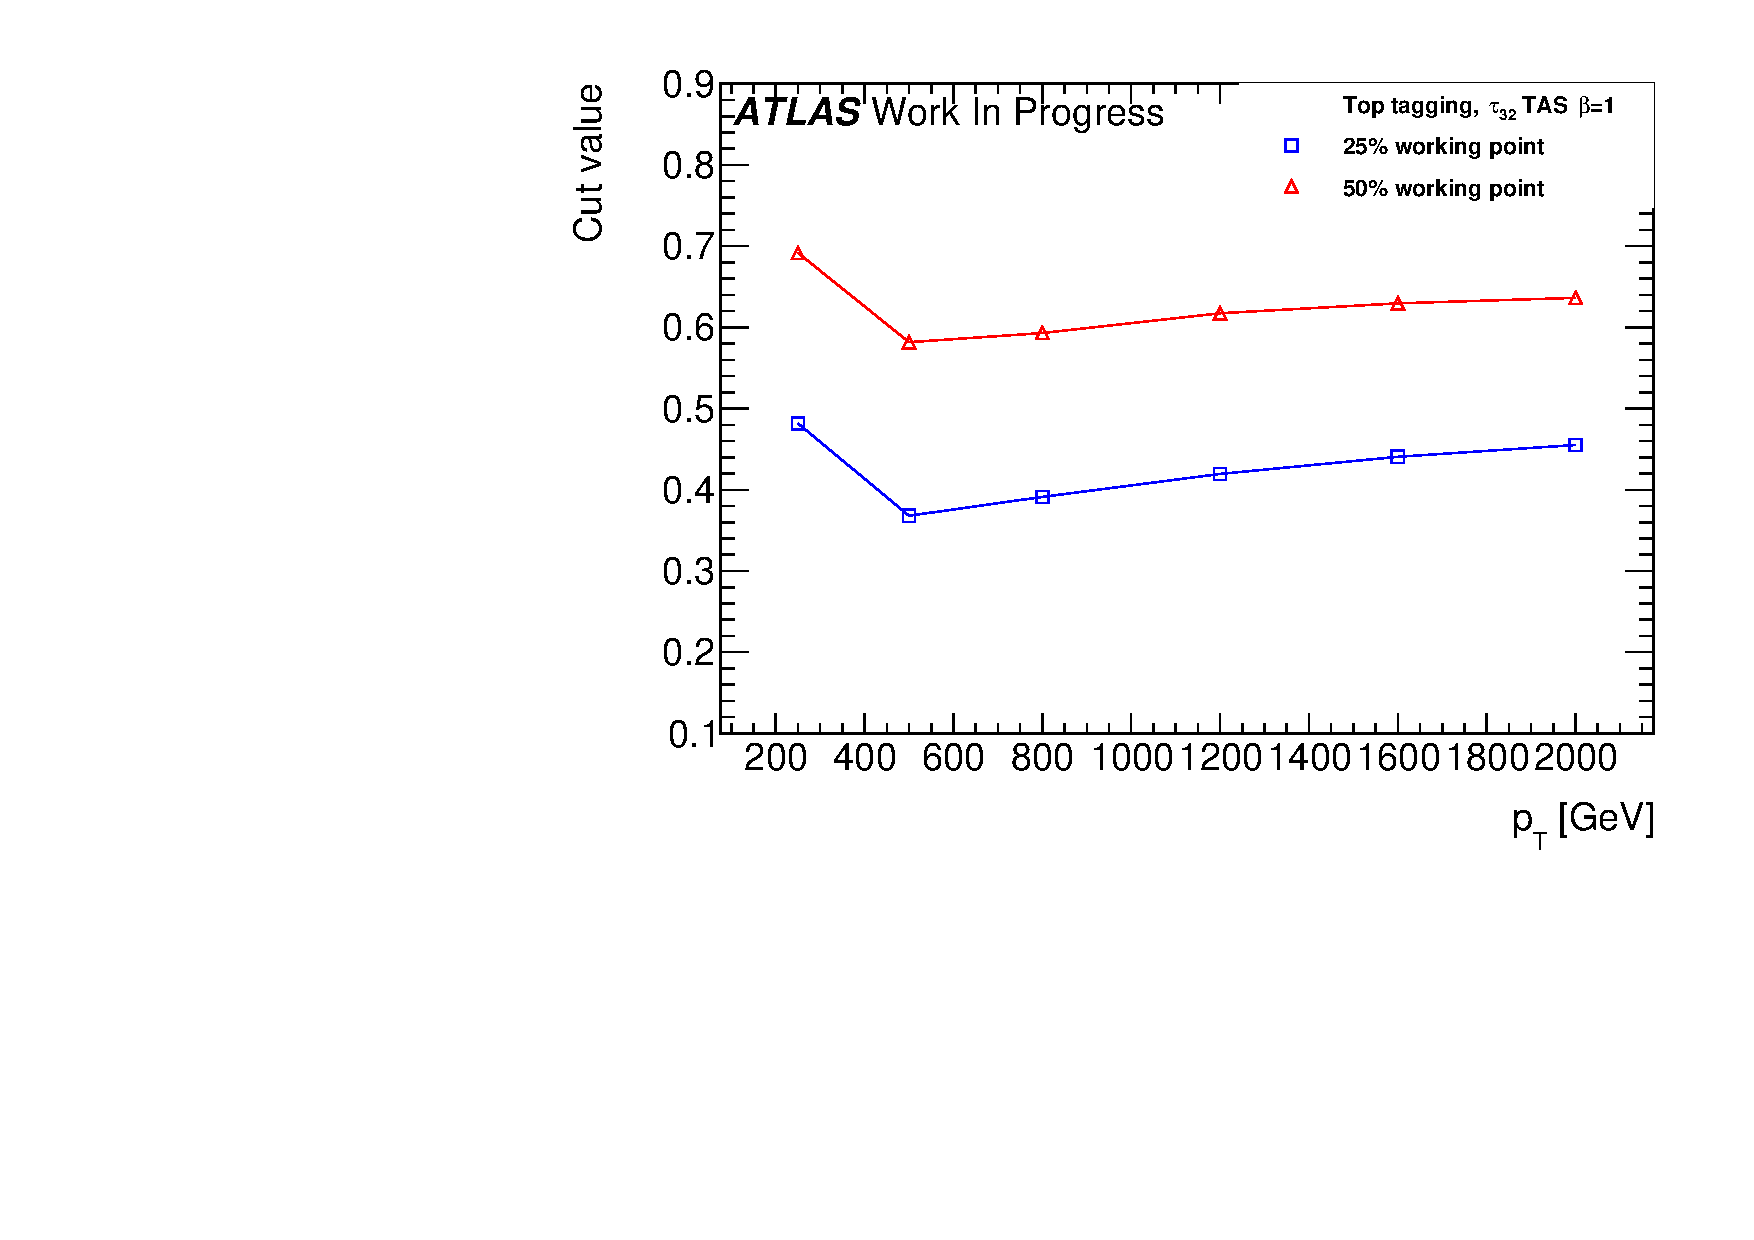
\includegraphics[width=0.5\textwidth]{sascha_input/plots/Top/cut_values/tau32_tas1.pdf} \hspace{1mm}
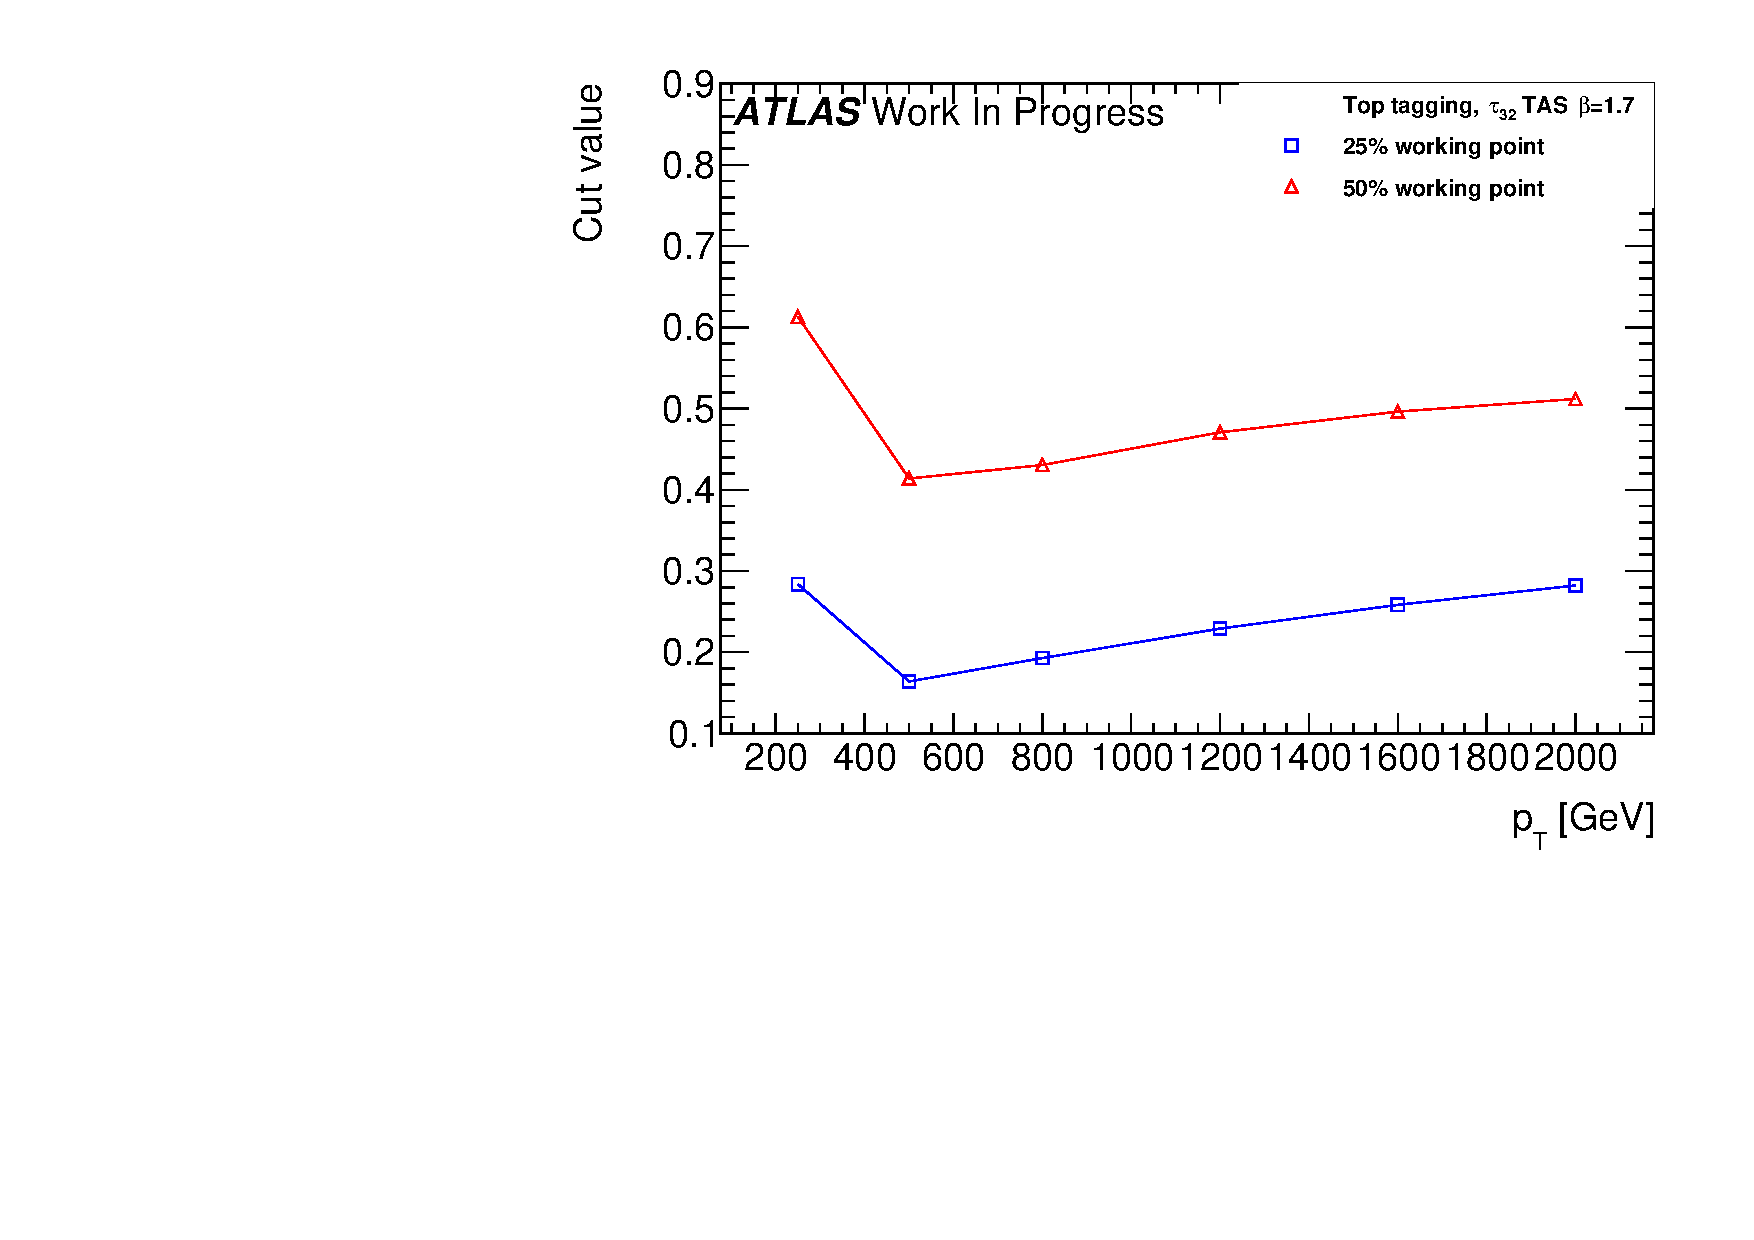
\includegraphics[width=0.5\textwidth]{sascha_input/plots/Top/cut_values/tau32_tas17.pdf}
\caption{\footnotesize{Cut values for $\tau_{32,\;\text{TAS}}^{(\beta=1)}$ (left) and $\tau_{32,\;\text{TAS}}^{(\beta=1.7)}$ (right) to achieve 50\% and 25\% Top quark efficiency}}\label{fig:top_cut}
\end{figure}

Listed in Table \ref{table:top_improvement} are the background rejections for $\tau_{32,\;\text{TAS}}^{(\beta=1)}$, $\tau_{32,\;\text{TAS}}^{(\beta=1.7)}$ and the best cluster based variable, $\tau_{32,\;\text{calo}}^{(\beta=2)}$. The differences between both values of $\beta$ with TAS are marginal, as well for lower signal efficiencies. Improvements due to the use of TAS instead of clusters are possible for Top quark tagging over the whole studied $p_{\mathrm{T}}$ range. These enhancements are, as expected, rising with the boost of the Top quark and can reach around $50\,\%$ for the $50\,\%$ working point and even $100\,\%$ for $25\,\%$ Top efficiency.
\begin{table}
\centering
\begin{tabular}{llll}
 \multicolumn{1}{l||}{\textbf{50\% $\epsilon_{signal}$}} &                                                & \textbf{Top Tagging}                                          &                                          \\ \hline
\multicolumn{1}{l||}{$p_{\mathrm{T}} \, \text{[GeV]}$}           & \multicolumn{1}{l|}{$\text{D2}_{\text{calo}}^{(\beta=2)}$} & \multicolumn{1}{l|}{$\tau_{32,\;\text{TAS}}^{(\beta=1)}$} & \multicolumn{1}{l|}{$\tau_{32,\;\text{TAS}}^{(\beta=1.7)}$} \\ \hline \hline
\multicolumn{1}{l||}{250 - 500}                       & \multicolumn{1}{l|}{9.5 $\pm$ 0.2}                      &  \multicolumn{1}{l|}{10.7 $\pm$ 0.2 (+13 $\pm$ 3 \%)}        & \multicolumn{1}{l|}{10.1 $\pm$ 0.2 (+6 $\pm$ 3 \%)}        \\
\multicolumn{1}{l||}{500 - 800}                       & \multicolumn{1}{l|}{22.4 $\pm$ 0.6}                      & \multicolumn{1}{l|}{22.8 $\pm$ 0.6 (+2 $\pm$ 4 \%)}         & \multicolumn{1}{l|}{22.8 $\pm$ 0.6 (+2 $\pm$ 4 \%)}         \\
\multicolumn{1}{l||}{800 - 1200}                      & \multicolumn{1}{l|}{20.6 $\pm$ 0.5}                      & \multicolumn{1}{l|}{23.6 $\pm$ 0.6 (+15 $\pm$ 4 \%)}        & \multicolumn{1}{l|}{24.1 $\pm$ 0.6 (+17 $\pm$ 4 \%)}        \\
\multicolumn{1}{l||}{1200 - 1600}                     & \multicolumn{1}{l|}{16.6 $\pm$ 0.4}                      & \multicolumn{1}{l|}{22.0 $\pm$ 0.6 (+33 $\pm$ 5 \%)}        & \multicolumn{1}{l|}{22.3 $\pm$ 0.6 (+34 $\pm$ 5 \%)}        \\
\multicolumn{1}{l||}{1600 - 2000}                     & \multicolumn{1}{l|}{13.3 $\pm$ 0.4}                      & \multicolumn{1}{l|}{18.9 $\pm$ 0.6 (+42 $\pm$ 6 \%)}        & \multicolumn{1}{l|}{18.8 $\pm$ 0.6 (+41 $\pm$ 6 \%)}       \\ 
\multicolumn{1}{l||}{$>2000$}                     	  & \multicolumn{1}{l|}{10.9 $\pm$ 0.4}                      & \multicolumn{1}{l|}{16.5 $\pm$ 0.7 (+51 $\pm$ 8 \%)}        & \multicolumn{1}{l|}{15.7 $\pm$ 0.7 (+44 $\pm$ 8 \%)}       \\ \hline
                                                     &                                                &                                          &                                          \\
 \multicolumn{1}{l||}{\textbf{25\% $\epsilon_{signal}$}} &                                                &  \textbf{Top Tagging}                                        &                                          \\ \hline
\multicolumn{1}{l||}{$p_{\mathrm{T}} \, \text{[GeV]}$}           & \multicolumn{1}{l|}{$\text{D2}_{\text{calo}}^{(\beta=2)}$} & \multicolumn{1}{l|}{$\tau_{32,\;\text{TAS}}^{(\beta=1)}$} & \multicolumn{1}{l|}{$\tau_{32,\;\text{TAS}}^{(\beta=1.7)}$} \\ \hline \hline
\multicolumn{1}{l||}{250 - 500}                       & \multicolumn{1}{l|}{33.7 $\pm$ 1.0}                     & \multicolumn{1}{l|}{37.6 $\pm$ 1.4 (+12 $\pm$ 5 \%)}       & \multicolumn{1}{l|}{36.7 $\pm$ 1.2 (+9 $\pm$ 5 \%)}       \\
\multicolumn{1}{l||}{500 - 800}                       & \multicolumn{1}{l|}{114.7 $\pm$ 3.3}                    & \multicolumn{1}{l|}{138.0 $\pm$ 4.3 (+20 $\pm$ 5 \%)}       & \multicolumn{1}{l|}{139.1 $\pm$ 4.2 (+21 $\pm$ 5 \%}        \\
\multicolumn{1}{l||}{800 -1200}                       & \multicolumn{1}{l|}{97.0 $\pm$ 2.7}                     & \multicolumn{1}{l|}{144.6 $\pm$ 4.9 (+49 $\pm$ 7 \%)}       & \multicolumn{1}{l|}{149.6 $\pm$ 5.2 (+54 $\pm$ 7 \%)}       \\
\multicolumn{1}{l||}{1200 - 1600}                     & \multicolumn{1}{l|}{68.6 $\pm$ 2.1}                     & \multicolumn{1}{l|}{133.2 $\pm$ 4.6 (+94 $\pm$ 9 \%)}       & \multicolumn{1}{l|}{134.7 $\pm$ 5.1 (+96 $\pm$ 10 \%)}      \\
\multicolumn{1}{l||}{1600 - 2000}                     & \multicolumn{1}{l|}{47.5 $\pm$ 1.6}                     & \multicolumn{1}{l|}{100.3 $\pm$ 4.2 (+111 $\pm$ 11 \%)}      & \multicolumn{1}{l|}{99.9 $\pm$ 4.4 (+110 $\pm$ 12 \%)}       \\ 
\multicolumn{1}{l||}{$>2000$}                         & \multicolumn{1}{l|}{36.3 $\pm$ 1.6}                     & \multicolumn{1}{l|}{80.2 $\pm$ 5.0 (+121 $\pm$ 17 \%)}      & \multicolumn{1}{l|}{75.5 $\pm$ 4.9 (+108 $\pm$ 16 \%)}       \\ \hline
\end{tabular}
\caption{Listing of the background rejections after the jet mass cut and tagging at 50\% and 25\% top signal efficiency for the identified best variables $\tau_{32,\;\text{TAS}}^{(\beta=1,1.7)}$ together with the improvements over the best variable with clusters which is $\text{D2}_{\text{calo}}^{(\beta=2)}$.}\label{table:top_improvement}
\end{table}



